% !TEX encoding = UTF-8 Unicode
% !TEX root = thesis-ex.tex

This chapter shall discuss some important experimental jet measurements that contextualize and motivate the study of the main analysis in this thesis.
These include the study of the hadron yields, dijet balance, jet yields, jet fragmentation, and jet profiles.

%\section{Common Kinematic Quantities}
%\label{sec:jet_kinematics}
%% !TEX encoding = UTF-8 Unicode
% !TEX root = thesis-ex.tex

This section defines some common quantities that are used throughout this thesis.

\subparagraph{Center of mass energy:}

\subparagraph{Energy and momentum:}
This analysis primarily deals with transverse momenta.
This is the projection of the momenta on the plane transverse to the beam axis. 
It is given by:

\begin{align}
\pt = |p| \sin\theta
\end{align}
\subparagraph{Rapidity and Pseudorapidity:}


%\section{Jet Reconstruction}
%\label{sec:jet_reconstruction}
%% !TEX root = thesis-ex.tex
Of the jet reconstruction algorithms that were discussed in Section~\ref{sec:jet_algo}, the LHC collaborations use the \antikt\ algorithm.
The ATLAS jet reconstruction procedure in heavy ion collisions is described in Ref.~\cite{2019108}, and is summarized in Figure~\ref{fig:atlasHIjetreco}.
It is different from the procedure for \pp\ collisions because of the large underlying event present in the heavy ion collision system.
%The heavy ion jet reconstruction procedure however, can also be applied to \pp\ collisions with ,

\begin{figure}[htbp!]
	\centering
	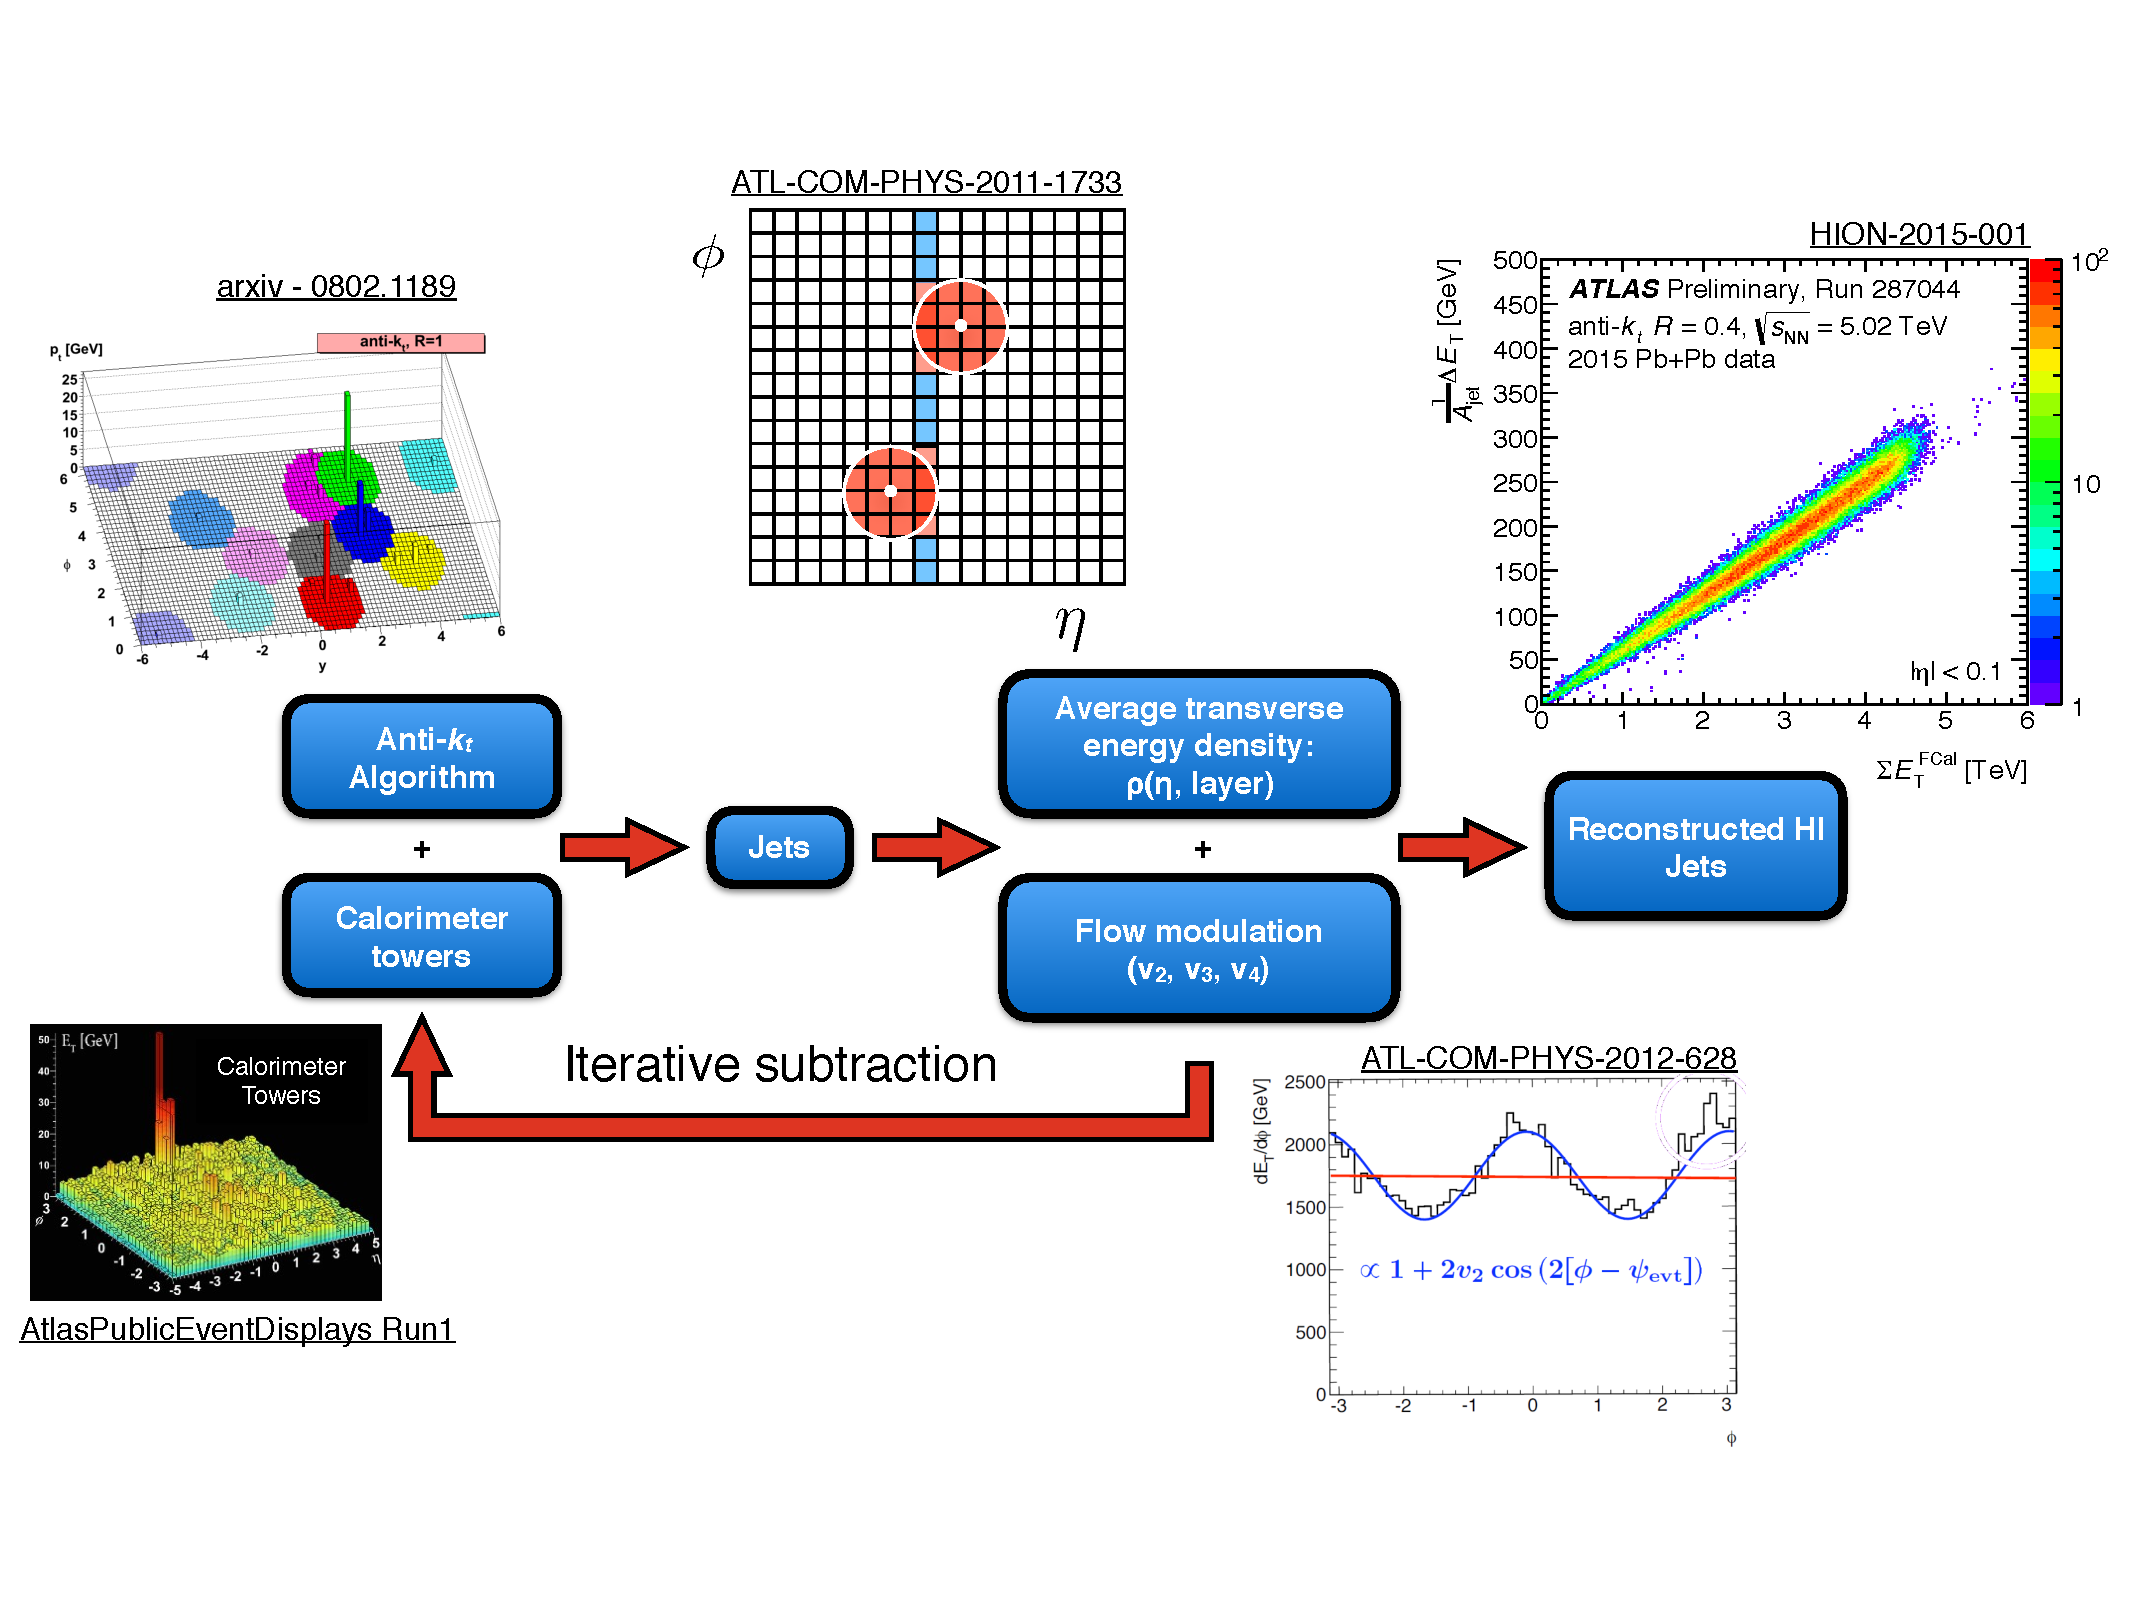
\includegraphics[width=0.7\textwidth]{figures/setup/atlasHIjetReco} %
	\caption{A schematic of the ATLAS jet reconstruction procedure.
	Inset figures from Refs.~\cite{Cacciari:2008gp, atlasRun1EventDisplay, ATLAS-COM-PHYS-2011-1733, Cole:1450219, perfPlots}.}	
	\label{fig:atlasHIjetreco}%
\end{figure}

This procedure uses the \antikt\ algorithm as implemented in \textsc{FastJet} software package \cite{fastjet_algo}.
The \antikt\ algorithm is run in four-momentum recombination mode with its inputs being the $\eta \times \phi = 0.1 \times \pi / 32$ calorimeter towers.
The tower energies are the sum of the energies of all layers in the tower with cells that straddle tower boundaries having their energies fractionally distributed.
The \antikt\ algorithm is first run with the distance parameter $R=0.2$, to give seed jets.

These seed jets contain at least one tower with $\Et > 3$ GeV, and have the ratio of the maximum tower transverse energy to the average tower transverse energy, $\Et^{Max} / \langle \Et \rangle > 4$.
Then the underlying event subtraction procedure is performed.
A first estimate of the average underlying event energy density $\rho_i (\eta)$ is done in 0.1 slices of $\eta$ in each calorimeter layer $i$ after excluding the regions that overlap with the seed jets.
A modulation is applied to account for the flow from the QGP (discussed in Section~\ref{sec:qgp_hi}) and the underlying event is subtracted to give $E_{Tj}^{\mathrm{sub}}$:

\begin{align}
E_{Tj}^{\mathrm{sub}} = E_{Tj} - A_j \rho_i (\eta_j) \Big(1+2 \sum_{n=2}^{4} {v_{n}}_i \big(\cos[2(\phi_j-\Psi_n)] \big) \Big)
\end{align}
where $E_{Tj} , \eta_j, \phi_j$ and $A_j$ are the cell $E_T, \eta, \phi$ and area for cell $j$ in layer $i$.
$v_{ni}$ are the $n^{\rm th}$ order harmonics of the modulation in layer $i$and are given by:

\begin{align}
v_{ni} = \frac{\sum_{j \in i} \Et_j \cos[2(\phi_j-\Psi_n)]}{\sum_{j \in i} \Et_j}
\end{align}
where the sum is over all cells $j$ in layer $i$.
$\Psi_n$ is the event plane angle and is given by \cite{ATLAS:2012at}:

\begin{align}
\Psi_n = \frac{1}{n} \tan^{-1} \left[ \frac{\langle \sum_k w_k \Et_k \sin(n\phi_k) \rangle}{\sum_k \Et_k \sin(n\phi_k)} \right]
\end{align}
where the sum is over all $k$ cells in the FCal and $\phi_k$ is the azimuthal angle of the cell.
The $w_k$ weights are to ensure a uniform $\Psi_n$ distribution.
The dominant effect in the modulation is from the second and third harmonic, $v_2$ and $v_3$ \cite{ATLAS:2012at}.

Once the background is subtracted, the \antikt\ algorithm is run again with the distance parameter $R = 0.2$.
The underlying event is re-estimated after excluding areas that are within $\Delta R = 0.4$ of the seeds.
Updated values of $\rho{'}_i$ and $v{'}_2$ are recalculated and used to estimate the background that is subtracted from the original cell energies.
This is then subtracted from the original cell energies to give kinematics for the $R= 0.4$ jets.
The average subtracted energy normalized by the area of the jet reconstructed jet, as a function of the energy in the forward calorimeter is shown in Fig~\ref{fig:subtr_energy}.
It can be seen that in the barrel region for $|\eta| < 0.1$, $R=0.4$ jets have a background that is approximately $300/(\pi\times 0.4^2) \approx 150$ GeV.
Figure~\ref{fig:jet_event_display} shows an ATLAS event display for a heavy ion collision with a reconstructed jet.


\begin{figure}
\centering
  \begin{minipage}{0.45\textwidth}
	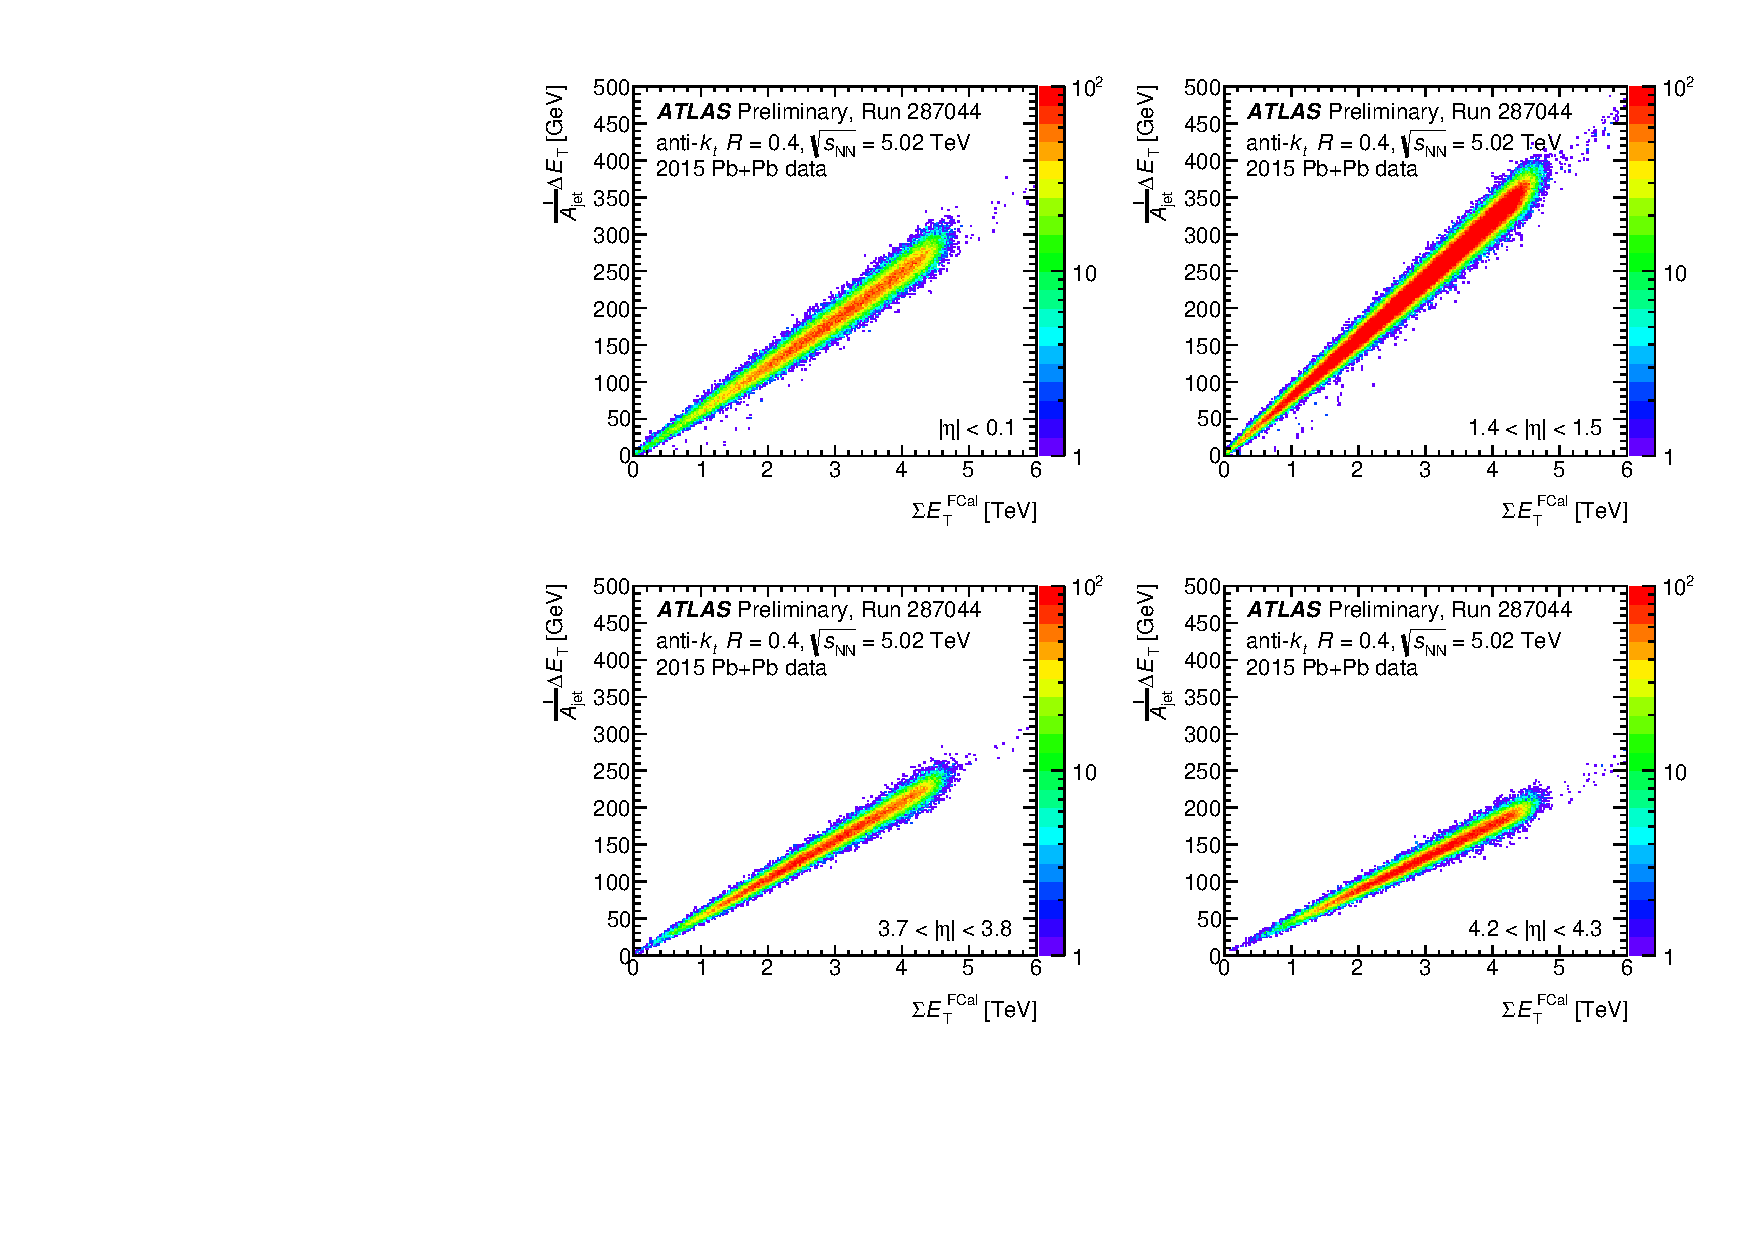
\includegraphics[width=1.\textwidth]{figures/setup/subtr_energy} %
	\caption{The subtracted transverse energy $\Delta \Et$, normalized by the jet area $A_{\rm{jet}}$ as a function of \ETfcal\ in \pbpb\ collisions at $\sqrtsnn = 5.02$ TeV.
	Figure from Ref.~\cite{perfPlots}.}	
	\label{fig:subtr_energy}
  \end{minipage}
 \qquad 
  \begin{minipage}{0.43\textwidth}
	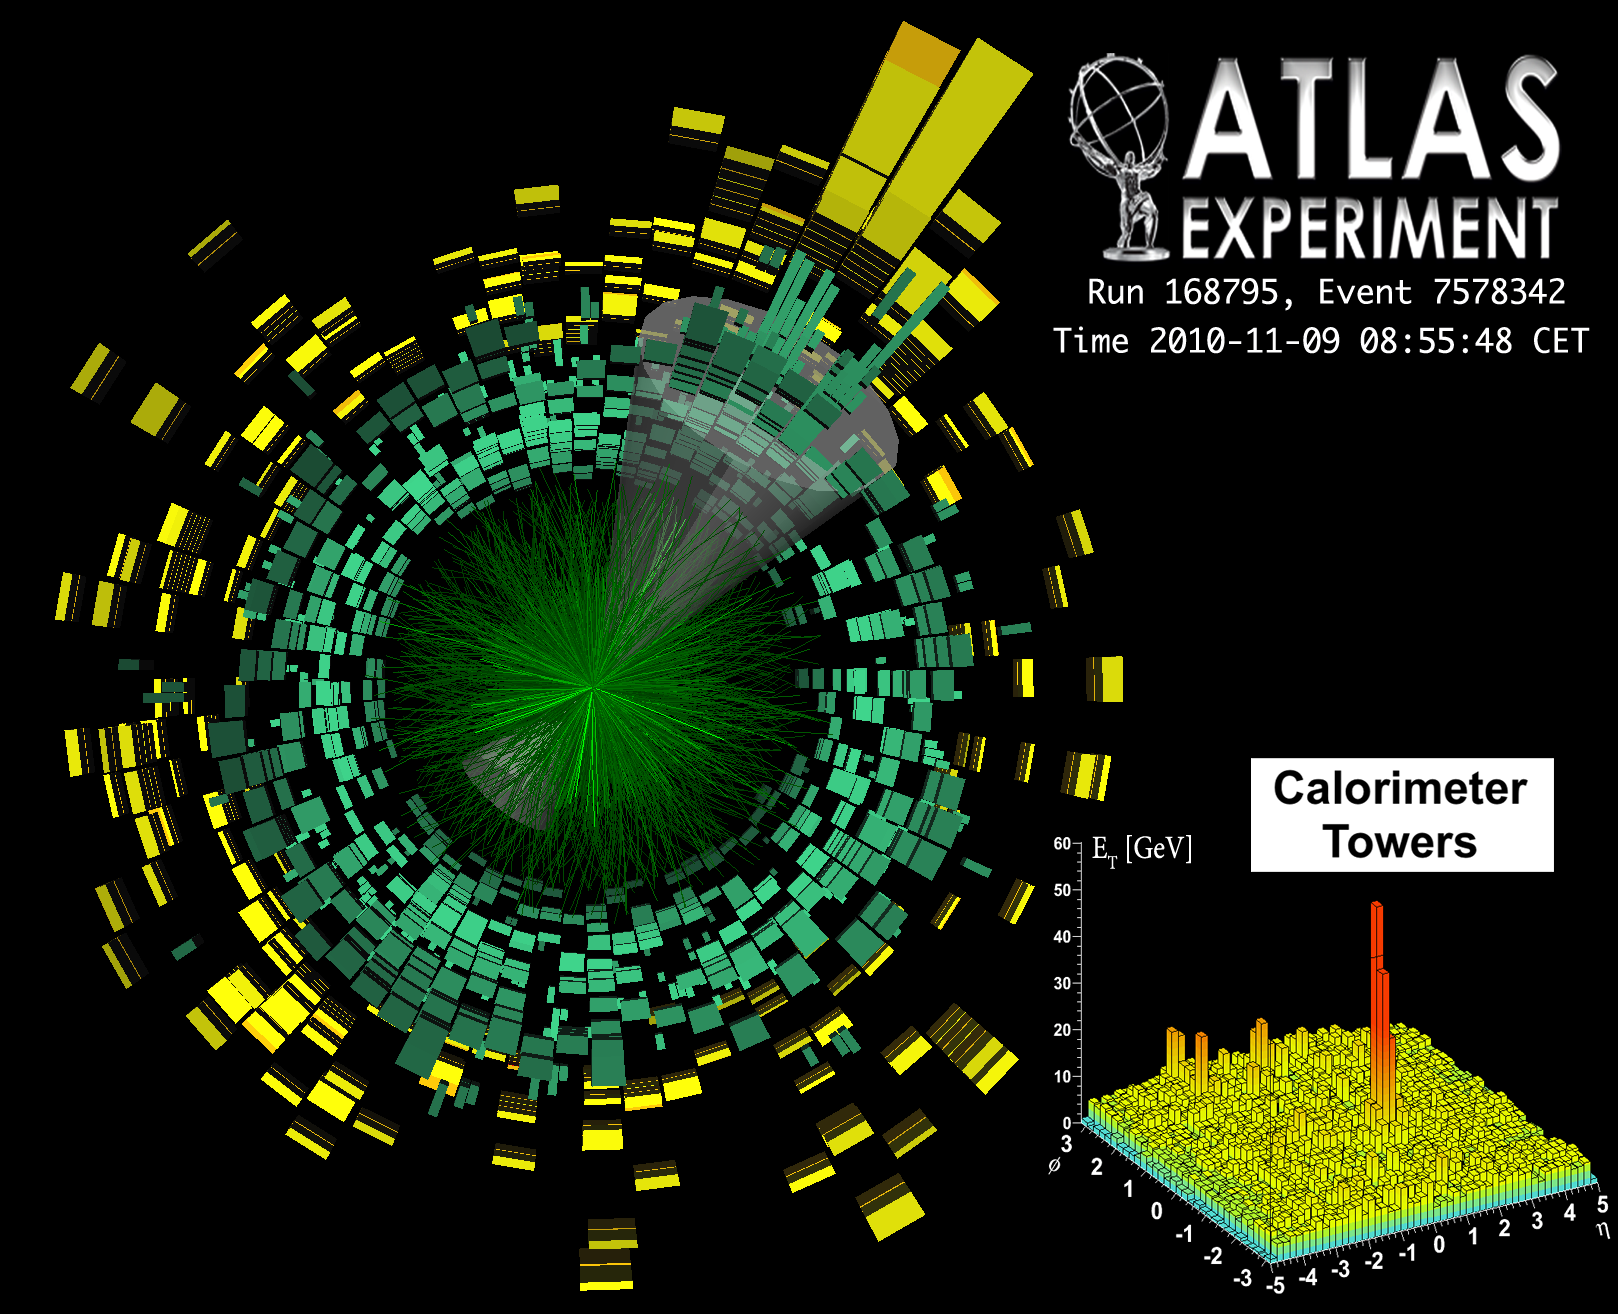
\includegraphics[width=1.\textwidth]{figures/setup/jet_event_display} %
	\caption{
	An asymmetric dijet event in \pbpb\ collisions at \sqrtsnn = 2.76 TeV as measured by the ATLAS detector. 
	Figure from Ref.~\cite{atlasRun1EventDisplay}.}	
	\label{fig:jet_event_display}
  \end{minipage}
\end{figure}



%
%\begin{figure}[htbp!]
%	\centering
%	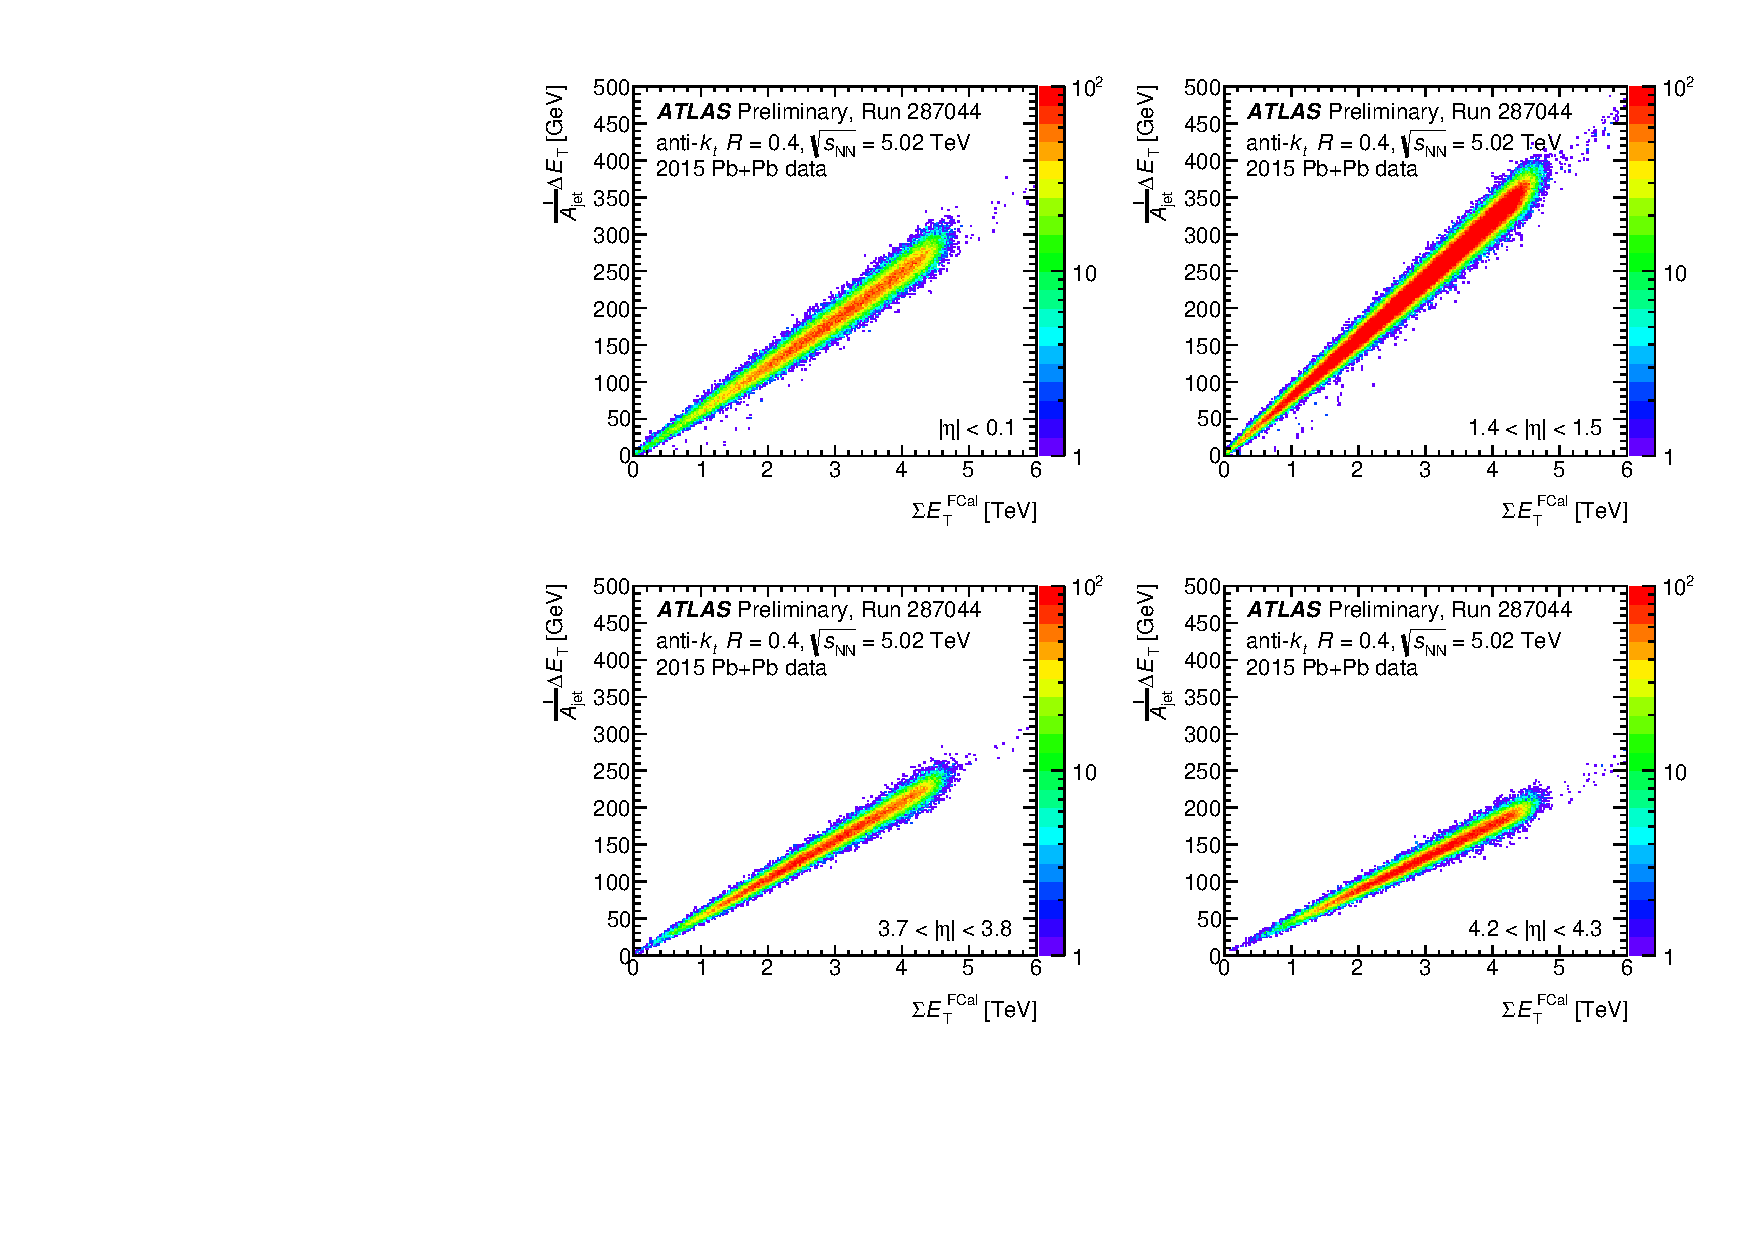
\includegraphics[width=0.5\textwidth]{figures/setup/subtr_energy} %
%	\caption{
%	The subtracted transverse energy $\Delta \Et$, normalized by the area of the jet $A_{\rm{jet}}$ as a function of the sum of the energy deposited in the forward calorimeter $\sum \Et_{\rm FCal}$ in \pbpb\ collisions at $\sqrtsnn = 5.02$ TeV.
%	The jets were reconstructed using the \antikt\ algorithm with $R = 0.4$.
%	Four panels show four selections on the pseudorapidity of the jet.
%	Figures taken from Ref.~\cite{perfPlots}.}	
%	\label{fig:subtr_energy}
%\end{figure}
%
%
%\begin{figure}[htbp!]
%	\centering
%	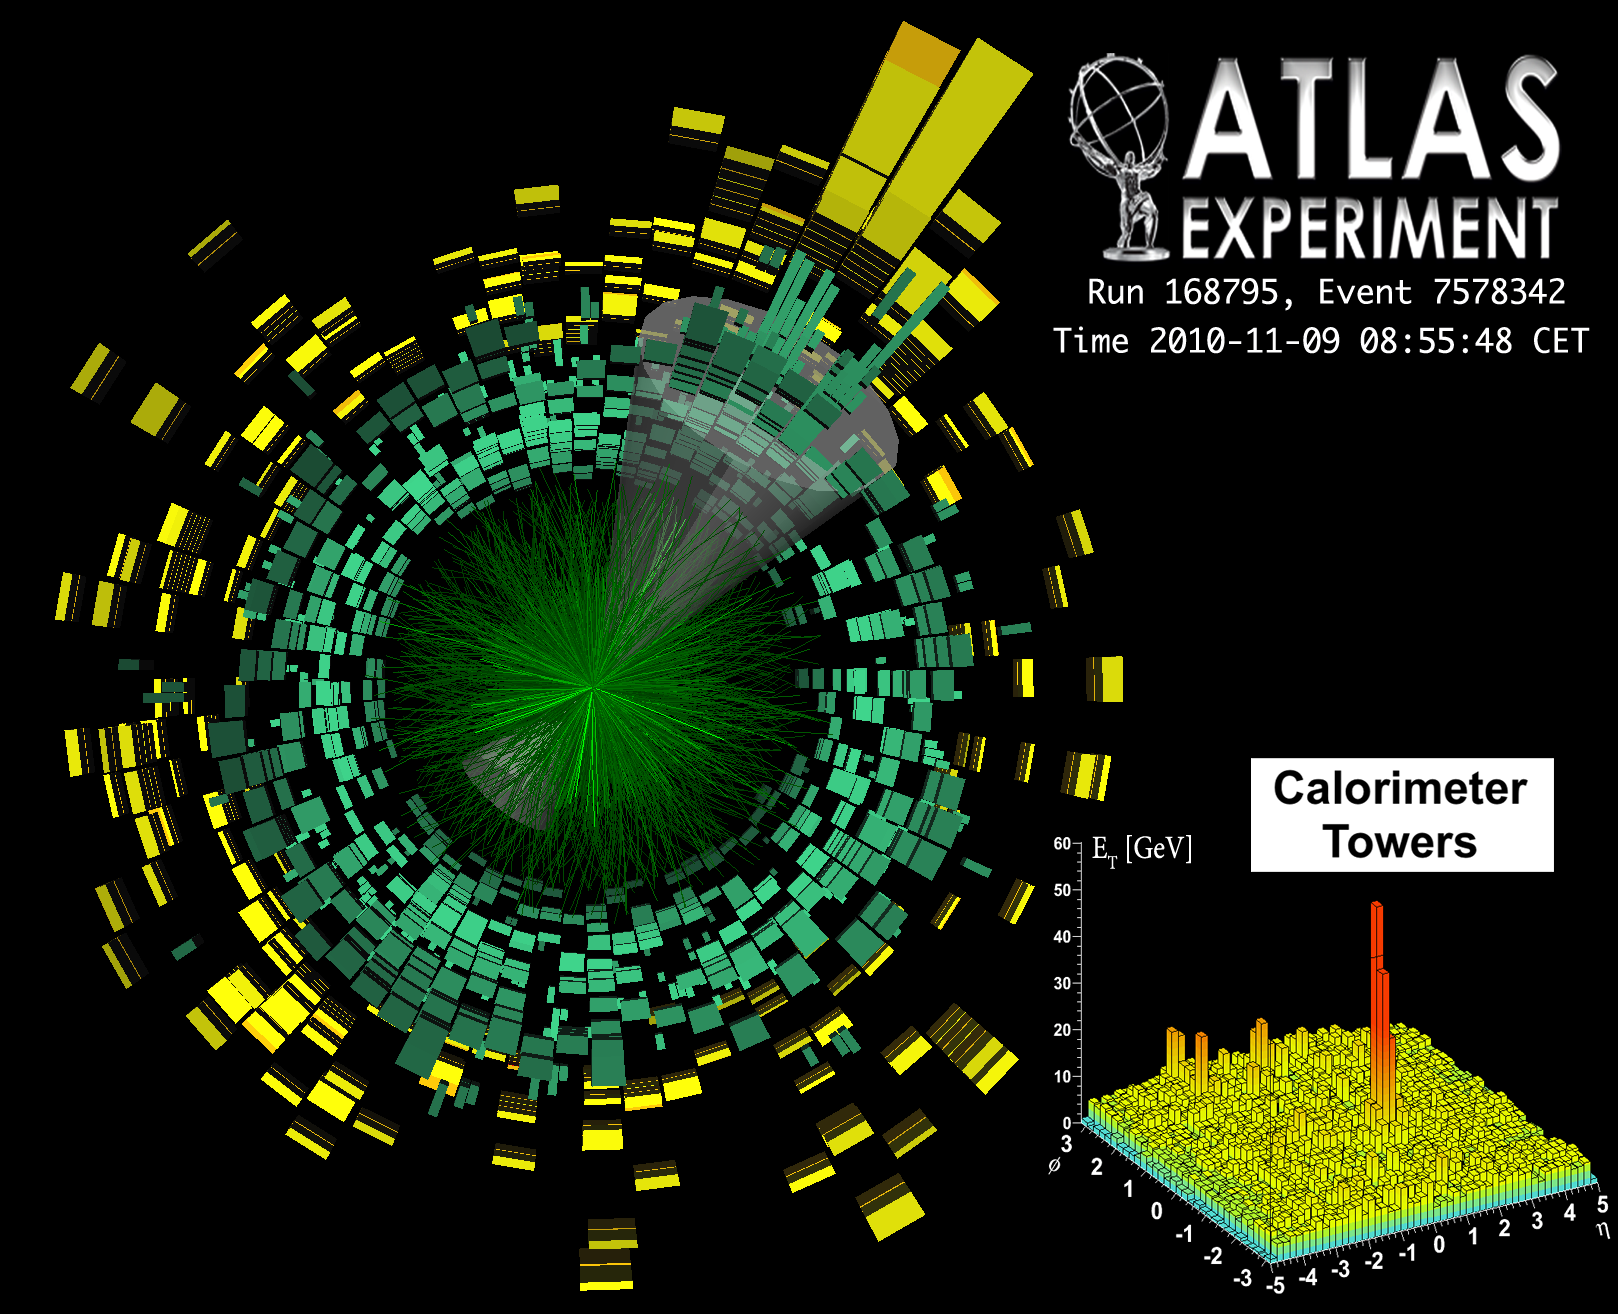
\includegraphics[width=0.5\textwidth]{figures/setup/jet_event_display} %
%	\caption{
%	An asymmetric dijet event in \pbpb\ collisions at \sqrtsnn = 2.76 TeV as measured by the ATLAS detector. 
%	Figures taken from Ref.~\cite{atlasRun1EventDisplay}.}	
%	\label{fig:jet_event_display}
%\end{figure}



\section{Hadron Suppresion}
\label{sec:hadron_suppresion}
% !TEX encoding = UTF-8 Unicode
% !TEX root = thesis-ex.tex


This discussion is based on Ref.~\cite{PhysRevLett.88.022301}.
Done at RHIC by the PHENIX collaboration, this was one of the first experimental measurements of jet quenching that showed the presence of the QGP.
This measurement analyzed high \pt\ charged hadrons and neutral $\pi^0$s ($\pt > 2$GeV) from jets produced in \AuAu\ collisions, collided at $\sqrtsnn = 130$ GeV.
Since jets form early in the collision and experience the evolution of the QGP, they are expected to lose energy due to collisional and radiative losses as discussed in Section~\ref{sec:jets}.
The modifications between the \pp\ and \AuAu\ system was quantified by constructing the nuclear modification factor \RAA, given as:

\begin{align}
\RAA_{\pt} = \frac{(1 / \Nevt) d^2 N^{\rm A+A} / d\pt d\eta}{(\langle N_{\rm binary} \rangle / \sigma_{\rm inel}^{\rm N+N} d^2 \sigma^{\rm N+N} / d\pt d\eta}
\end{align}
where \Nevt\ is the number of \AuAu\ events, $\langle N_{\rm binary} \rangle$ is the average number of binary collisions per event, $\sigma$ is the scattering cross section, and \pt\ and $\eta$ are the kinematics of the charged particle.
The \RAA\ for charged hadrons and neutral pions is shown in Figure~\ref{fig:hadron_raa}.

\begin{figure}
\begin{subfigure}{.49\textwidth}
  \centering
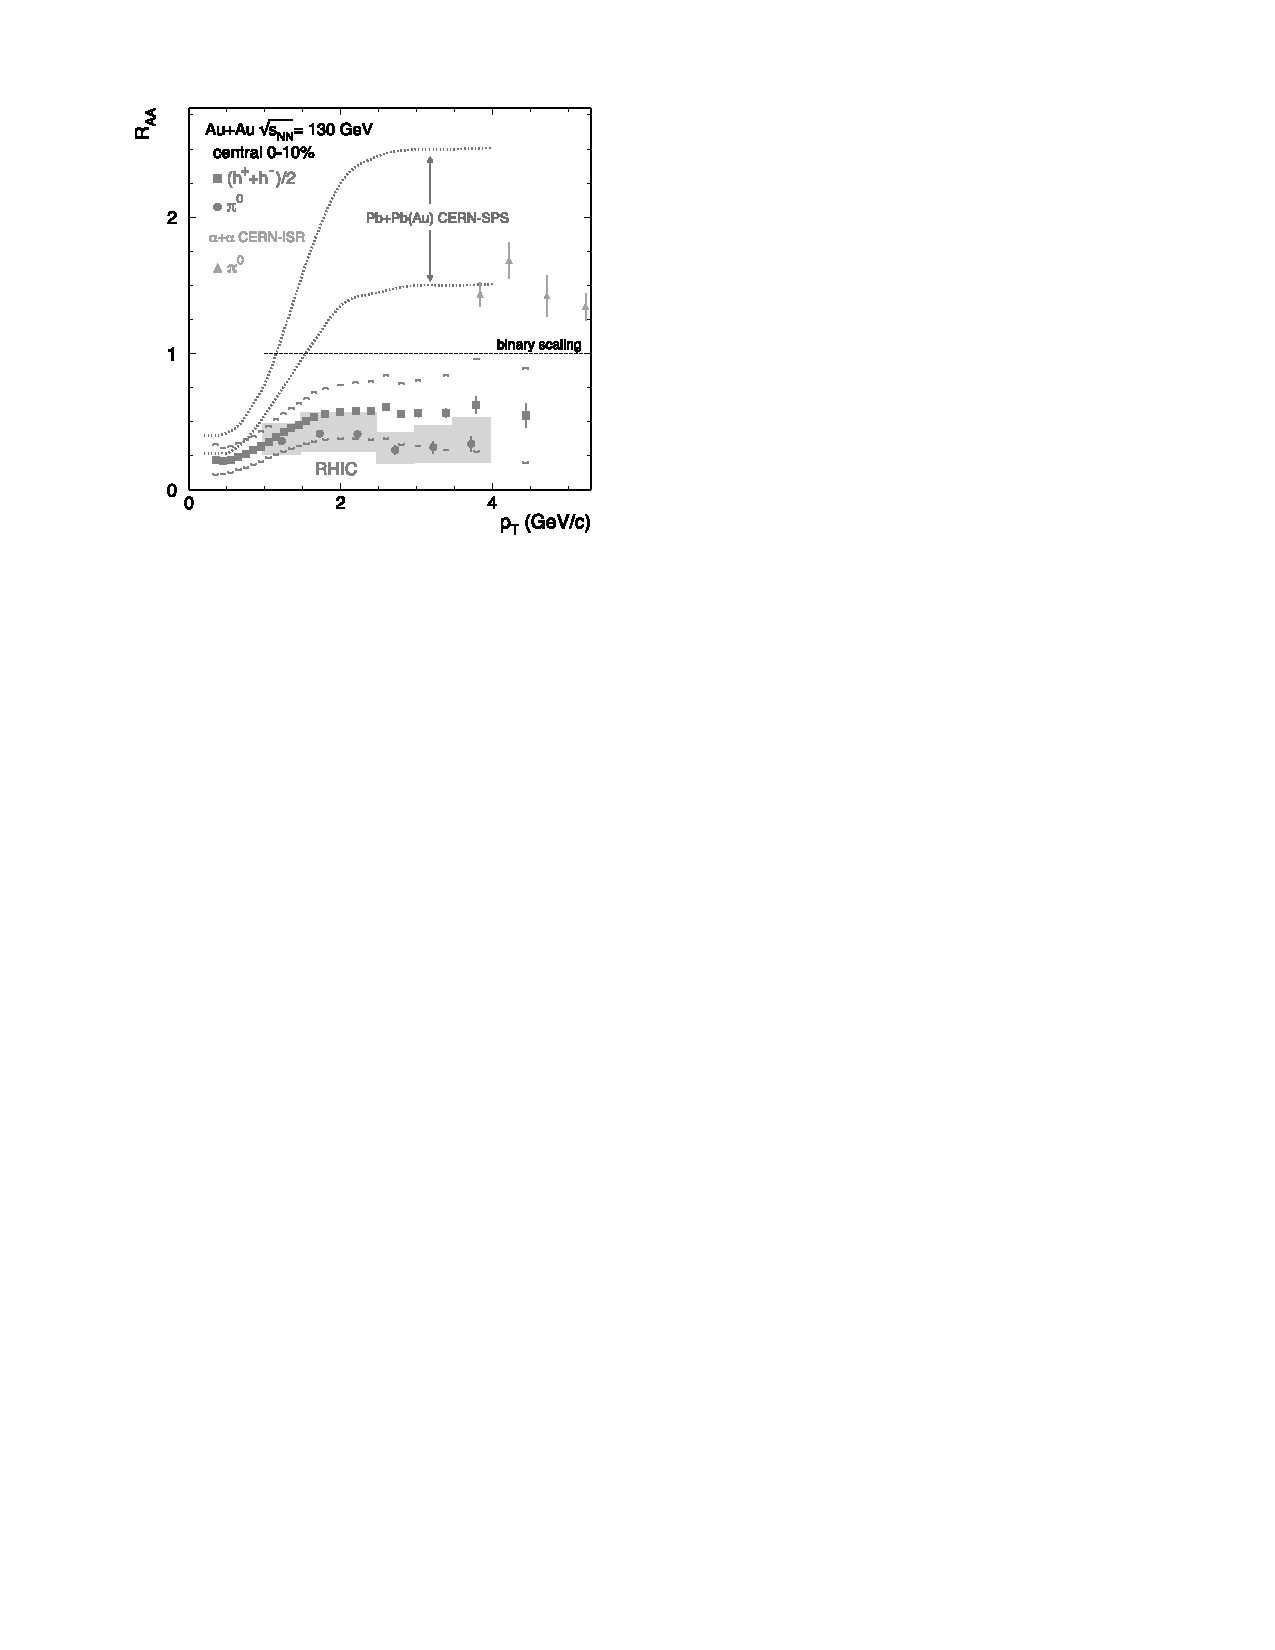
\includegraphics[width=\textwidth]{figures/jetMeasurements/hadron_raa}
\caption{The \RAA\ for charged hadrons and neutral pions in \AuAu\ collisions at $\sqrtsnn = 130$ GeV.
Also shown is the \RAA\ for inclusive cross sections in $\alpha+\alpha$ compared to \pp\ at $\sqrtsnn = 31$ GeV \cite{ANGELIS1987213} and spectra from \pbpb and $\rm{Pb}+{\rm AU}$ compared to \pp\ at $\sqrtsnn = 17$ GeV \cite{PhysRevC.64.034901}.
Figure taken from Ref.~\cite{PhysRevLett.88.022301}.}
\label{fig:hadron_raa}
\end{subfigure} \qquad
\begin{subfigure}{.49\textwidth}
  \centering
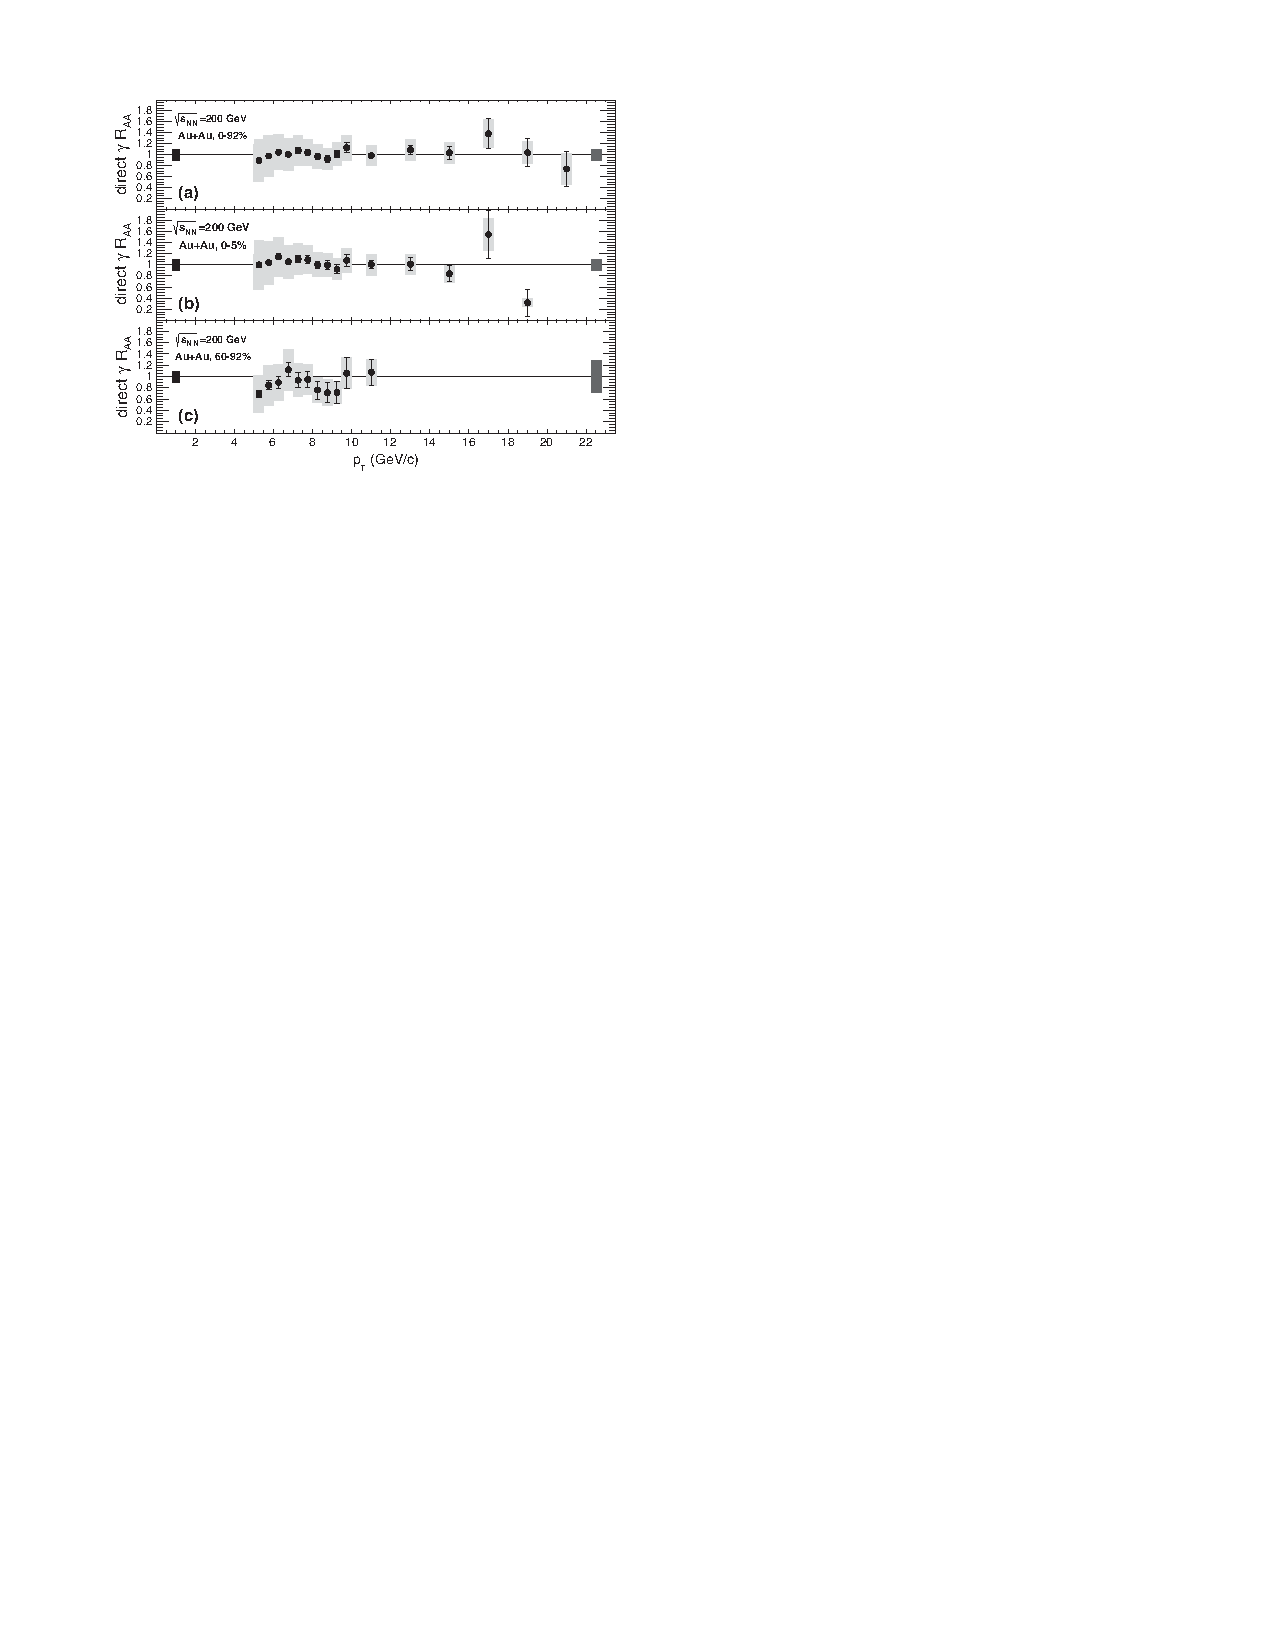
\includegraphics[width=\textwidth]{figures/jetMeasurements/photon_raa}
\caption{The \RAA\ for photons in three centrality regions in \AuAu\ collisions at $\sqrtsnn = 200$ GeV.
Figure taken from Ref.~\cite{PhysRevLett.109.152302}.}
\label{fig:photon_raa}
\end{subfigure}
\caption{\RAA\ evaluated for (left) charged hadrons and pions and (right) photons.}
\label{fig:particle_raa}
\end{figure}


%\begin{figure}[htbp]
%\begin{center}
%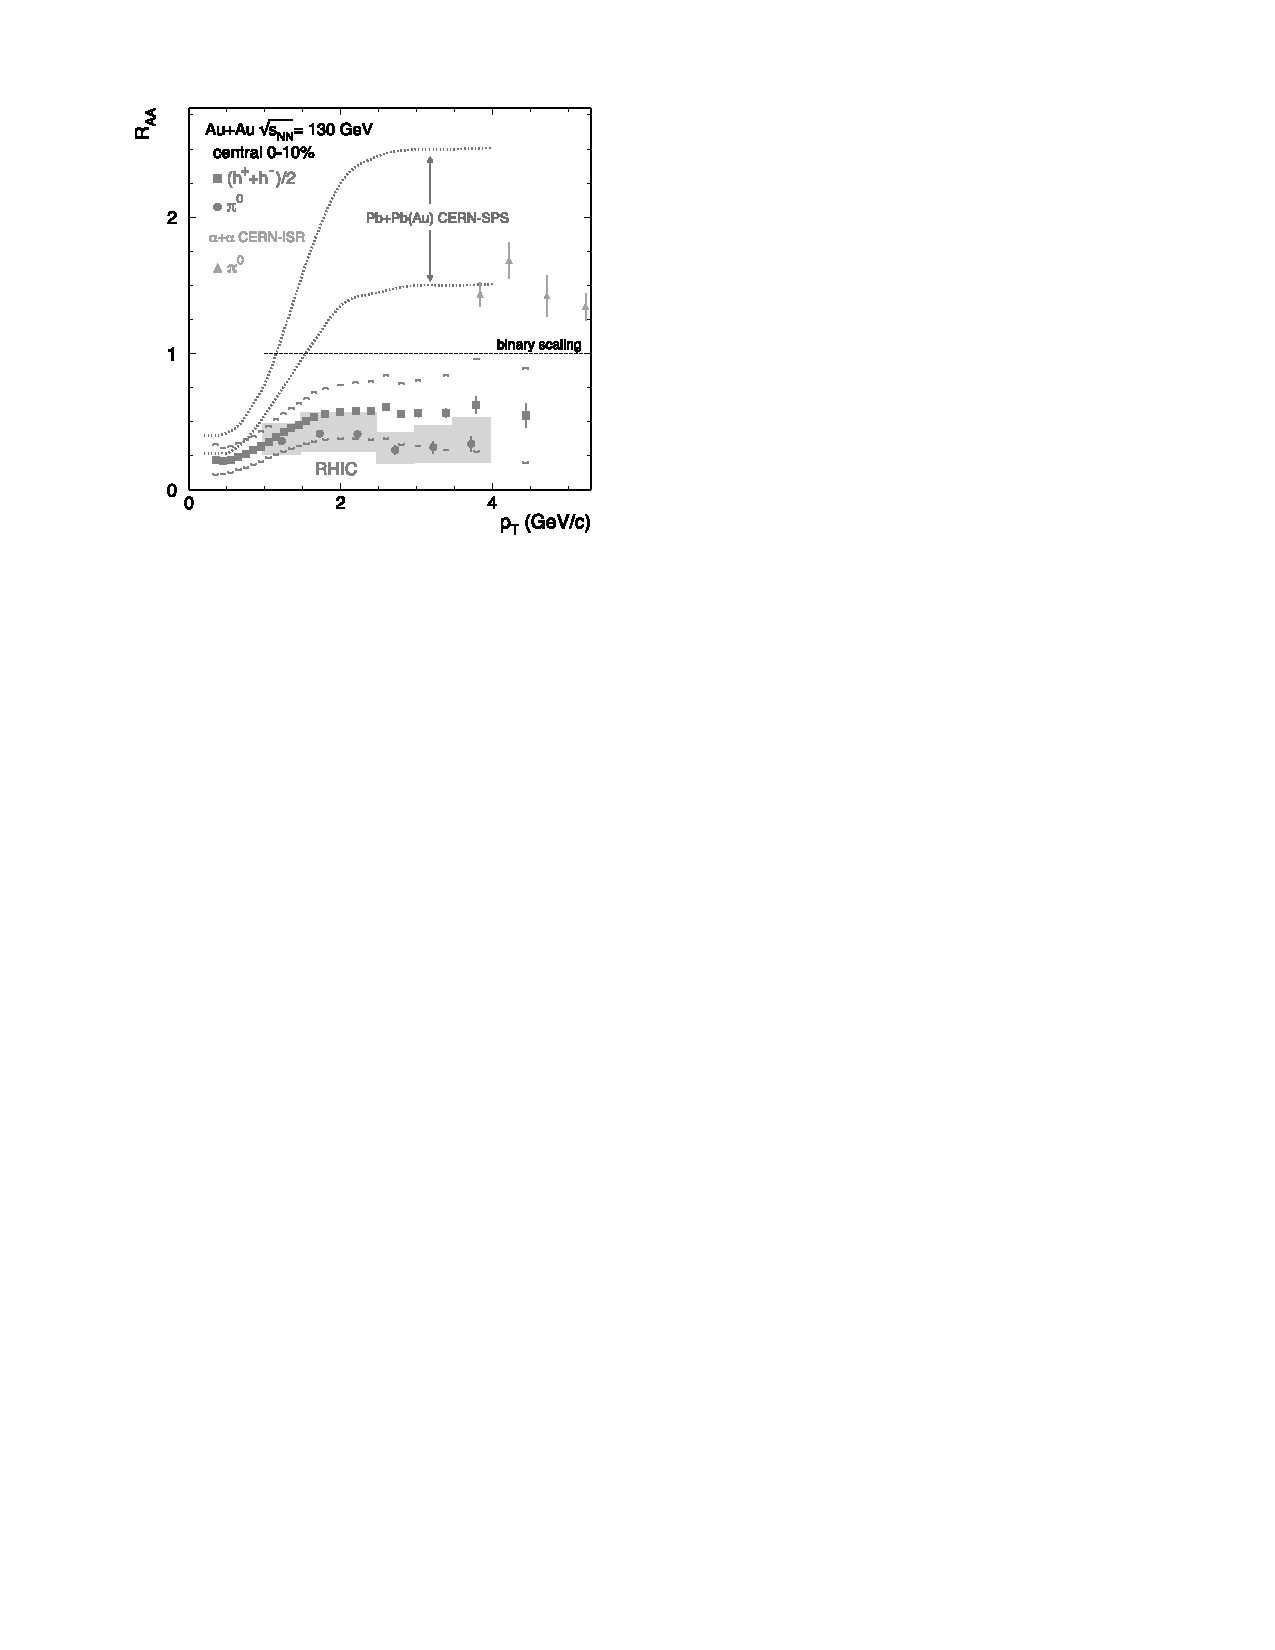
\includegraphics[width=0.55\textwidth]{figures/jetMeasurements/hadron_raa}
%\caption{The \RAA\ for charged hadrons and neutral pions in \AuAu\ collisions at $\sqrtsnn = 130$ GeV.
%Also shown is the \RAA\ for inclusive cross sections in $\alpha+\alpha$ compared to \pp\ at $\sqrtsnn = 31$ GeV \cite{ANGELIS1987213} and spectra from \pbpb and $\rm{Pb}+{\rm AU}$ compared to \pp\ at $\sqrtsnn = 17$ GeV \cite{PhysRevC.64.034901}.
%Figure taken from Ref.~\cite{PhysRevLett.88.022301}.}
%\label{fig:hadron_raa}
%\end{center}
%\end{figure}

A significant depletion is seen, with the \RAA\ rising for $\pt < 2$ GeV and remaining fairly constant thereafter.
This modification includes both hot nuclear matter effects from the QGP, as well as cold nuclear matter effects like the Cronin effect that can be seen in $p+A$ collisions \cite{PhysRevD.19.764}.

Electroweak probes like photons and Z bosons do not lose energy is the QGP since they do not interact strongly, and their \RAA\ is expected to be closer to unity.
There can be differences though, that are coming from cold nuclear matter effects.
This can be seen in Figure~\ref{fig:photon_raa}

\section{Dijet Balance: $\mathrm{x}_{J}$}
\label{sec:xj}
% !TEX encoding = UTF-8 Unicode
% !TEX root = thesis-ex.tex

This section will discuss the dijet balance for $R = 0.4$ jets as measured by ATLAS detector for \pbpb\ collisions at \sqrtsnn = 2.76 TeV \cite{Aaboud:2017eww}.
The dijet imbalance can be expressed in terms of $x_J$ defined as

\begin{align}
x_J =  \frac{\pt_2}{\pt_1}
\end{align}
where $\pt_2$ and $\pt_1$ are the transverse momenta of the two highest-\pt\ jets in the event respectively.
The minimum $\pt_2$ considered is 25 GeV and the pair of jets are separated by $|\Delta\phi| > 7\pi/8$.
The dijet yields normalized by the number of jets and determined as $1/N_\mathrm{jets} dN/dx_J$ are presented as a function of $x_J$ for different centrality intervals, as well as different ranges for $\pt_1$.
The measured distributions are further unfolded to remove detector resolution effects and allow comparison to theoretical models.

Figure~\ref{fig:xJ} shows the $x_J$ distribution for dijet pairs in \pp\ and \pbpb\ collisions in two different centrality bins and two $\pt_1$ ranges.
It can be seen that the dijet yields in \pp\ are peaked at unity and become narrower for larger $\pt_1$ ranges.
This reflects the fact that the effects of jet quenching are minimal and the higher-\pt\ jets are better balanced.
The dijet yields in peripheral \pbpb\ collisions are similar to the distributions from the \pp\ data, showing that the effects of quenching are smaller.
On the other hand, dijet yields in central \pbpb\ collisions are significantly broadened, reflecting the maximal  of jet quenching.
This is consistent with the picture of the individual jets in the dijet pair traversing different lengths in the QGP and hence losing different amounts of energy.
In fact, the distribution for \pbpb\ data is peaked at $x_J = 0.5$, implying a loss of 50\% of the jet \pt.

\begin{figure}[htbp]
\begin{center}
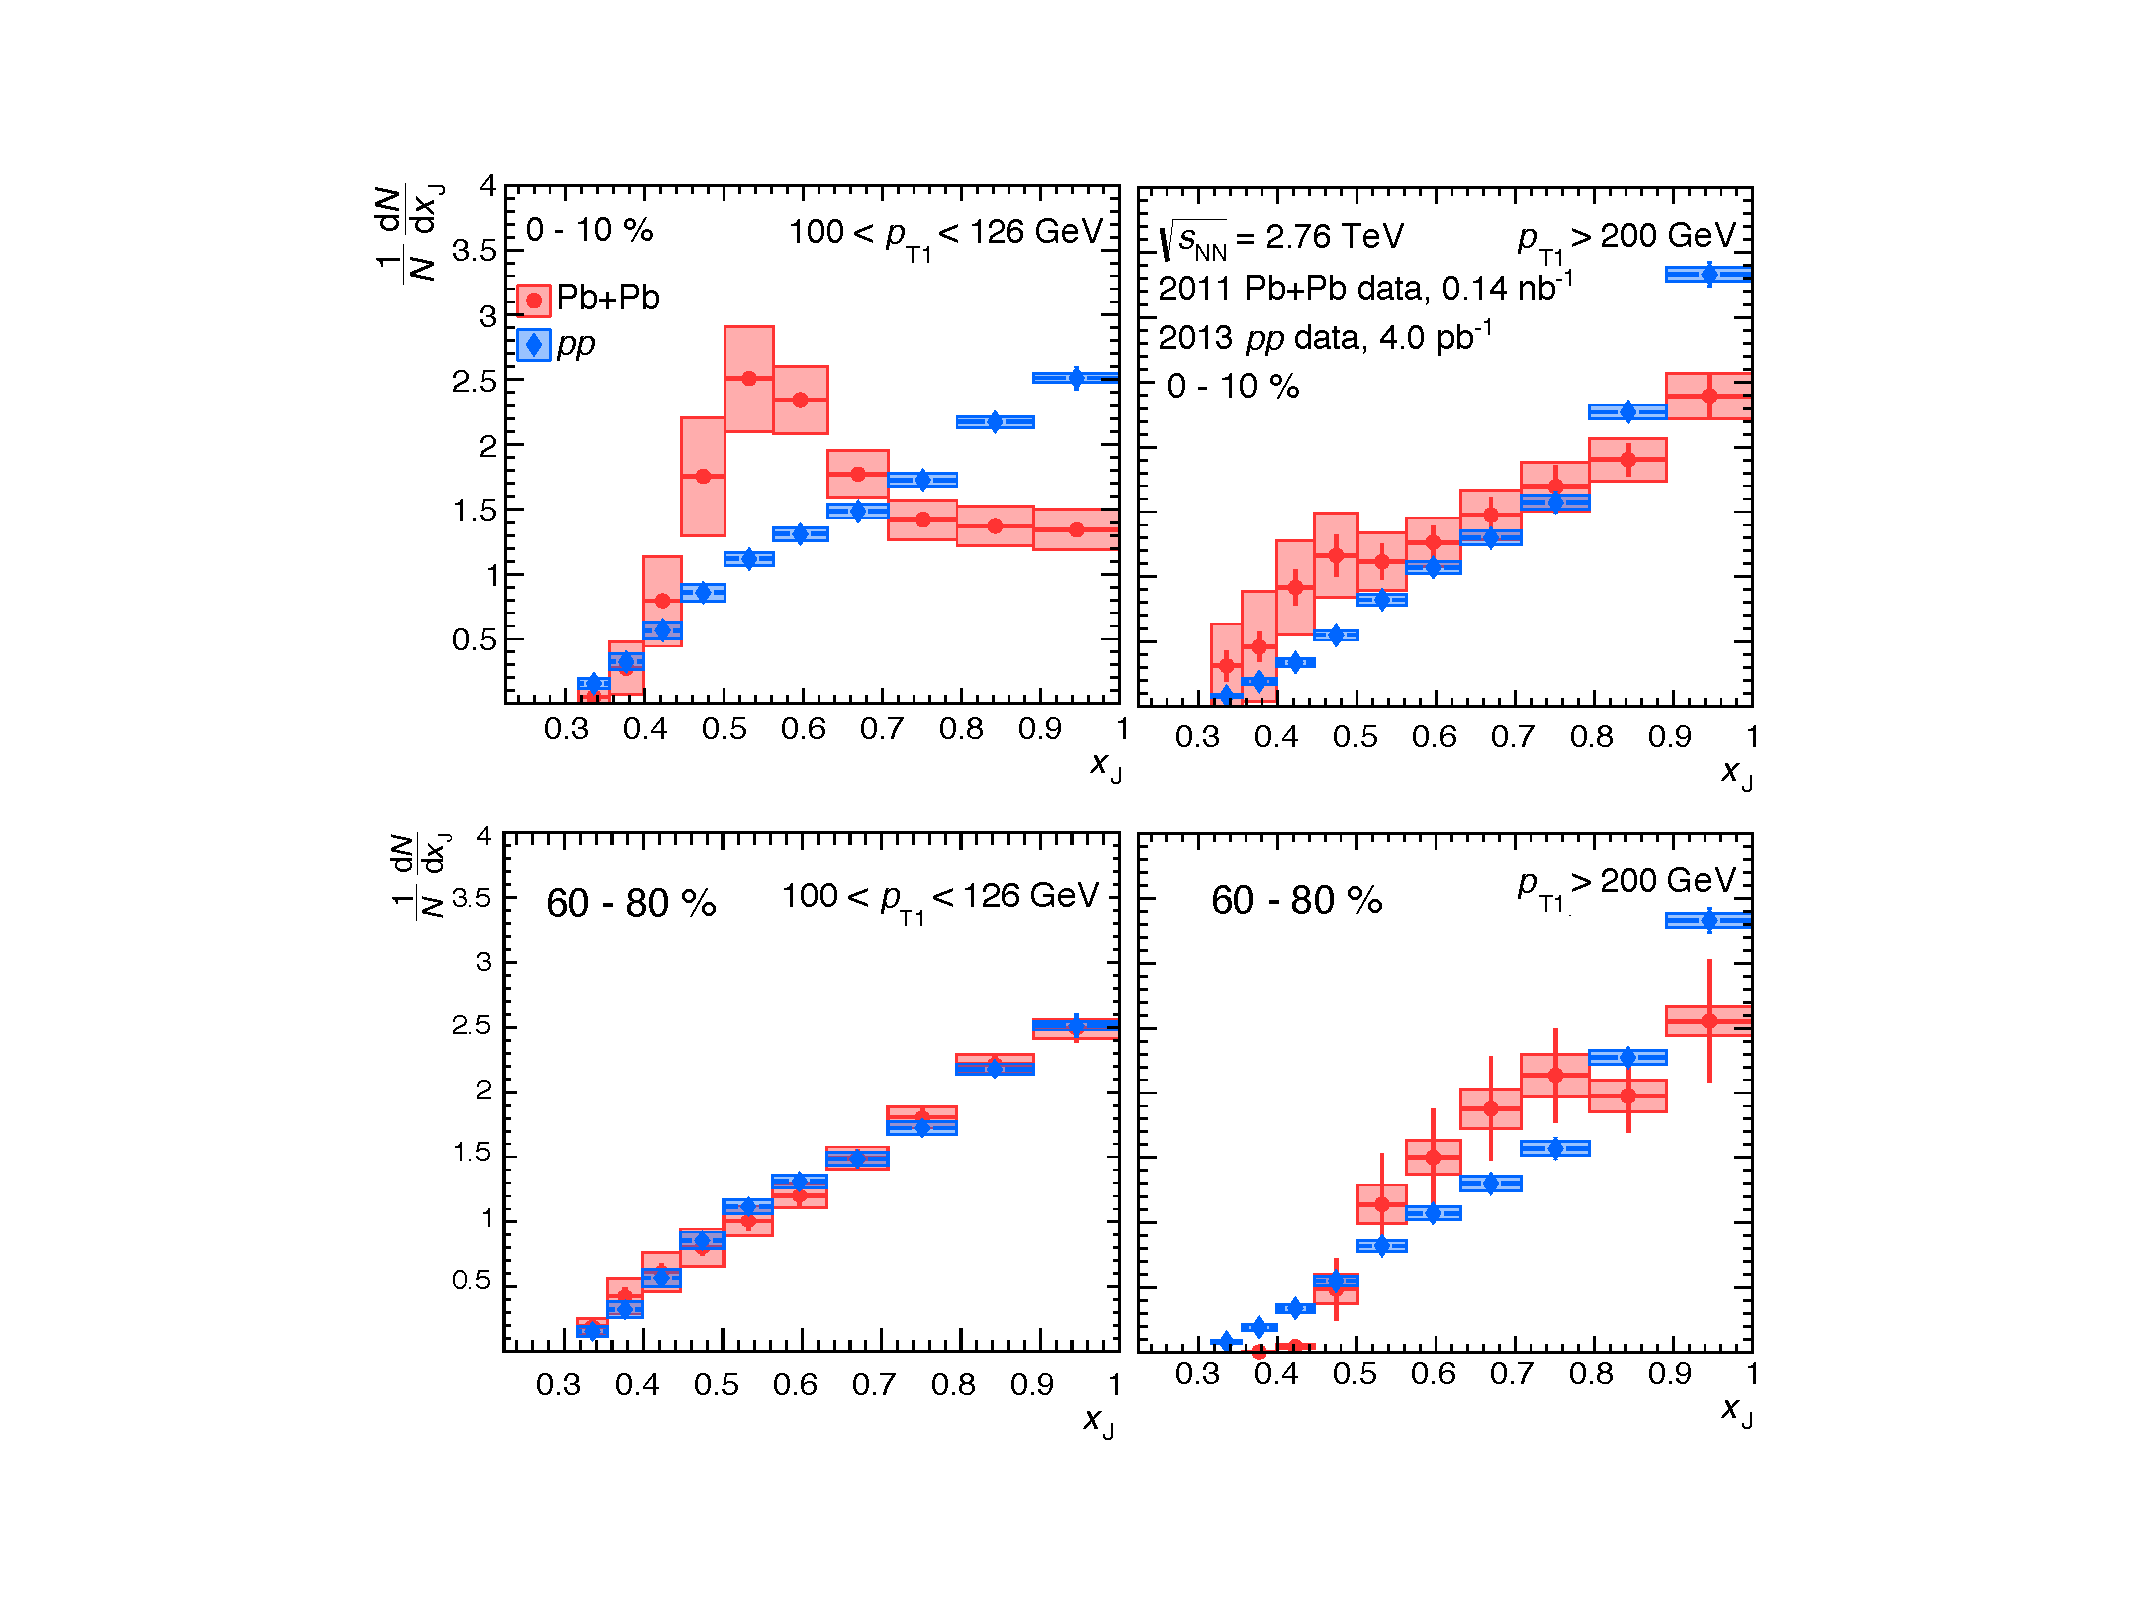
\includegraphics[width=0.55\textwidth]{figures/jetMeasurements/xJ}
\caption{The $1/N_\mathrm{jets} dN/dx_J$ distributions for $R=0.4$ jets as a function of $x_J$ for \pp\ (blue) and \pbpb\ (red) collisions.
The different panels are for (top) central and (bottom) peripheral collisions in (left) $100 < \pt_1 < 126$ GeV and (right) $\pt_1 > 200 $ GeV.
The \pp\ data is the same in all panels.
The statistical uncertainties are indicated by the bars while the boxes indicate the systematic uncertainties.
Figures taken from \cite{Aaboud:2017eww}.}
\label{fig:xJ}
\end{center}
\end{figure}

Further measurements of $R = 0.3$ jets are shown in Figure~\ref{fig:xJ_R03}.
These distributions are significantly flatter than the ones for $R=0.4$ jets, an observation that is consistent with the expectation that the transverse momenta correlation between the dijet pair is weaker for jets with smaller radii due to radiation that is outside the nominal jet cone.

\begin{figure}[htbp]
\begin{center}
\includegraphics[width=0.55\textwidth]{figures/jetMeasurements/xJ_R03}
\caption{The $1/N_\mathrm{jets} dN/dx_J$ distributions for $R=0.3$ jets as a function of $x_J$ in \pp\ and central \pbpb\ collisions.
The different panels are for different, $\pt_1$ ranges (top left to bottom right) central and (bottom) peripheral collisions.
The \pbpb\ data is in red circles while the \pp\ data is in blue diamonds and is the same in all panels.
The statistical uncertainties are indicated by the bars while the boxes indicate the systematic uncertainties.
Figures taken from \cite{Aaboud:2017eww}.}
\label{fig:xJ_R03}
\end{center}
\end{figure}



\section{Modification of jet yields: $\mathrm{R}_{AA}$}
\label{sec:jet_raa}
% !TEX encoding = UTF-8 Unicode
% !TEX root = thesis-ex.tex

This section discusses the measurement of the inclusive jet \RAA\ as measured by the ALICE detector for jets in $\sqrtsnn=2.76$ TeV \pbpb\ and \pp\ collisions \cite{Reed_2013}.

While measurements that compare jets in a dijet system to each other as discussed in Section~\ref{sec:xj} can provide valuable information about how jets lose energy, they have the following limitation: If both jets lose equal amounts of energy, the dijet yield will still be peaked at unity and no new information will be obtained.
Thus, it is useful to compare the jet yields directly between the \pp\ and \pbpb\ systems and construct the jet \RAA\ observable.
This is defined as:

\begin{align}
\RAA  = \dfrac{\dfrac{1}{N_{\rm evt}} \left.
\dfrac{d^2 N_{\rm jet}}{d\pt dy} \right|_{\rm cent}}{ \langle T_{\rm AA} \rangle \left.
\dfrac{d^2\sigma_{\rm jet}}{d\pt dy} \right|_{\rm pp}}
\end{align}
where \TAA\ is the nuclear thickness function and accounts for the geometric enhancement between \pp\ and \pbpb\ as discussed in Section~\ref{sec:qgp_hi} and \cite{doi:10.1146/annurev.nucl.57.090506.123020}.

This measurement includes considers jets from both charged particles and neutral $\pi^0$s.
The jet spectrum in \pbpb\ events, as well as the jet \RAA\ for central \pbpb\ is shown in Figure~\ref{fig:jet_raa_alice}.
It can be seen that the most central collisions show a clear suppression with an $\RAA \approx 0.25$ at jet $\pt\ 30$ GeV.
The \RAA\ value slowly evolves with jet \pt\ and rises to 0.5 at jet $\pt = 100$ GeV.
This modification becomes smaller for more peripheral collisions.

\begin{figure}[htbp]
\begin{center}
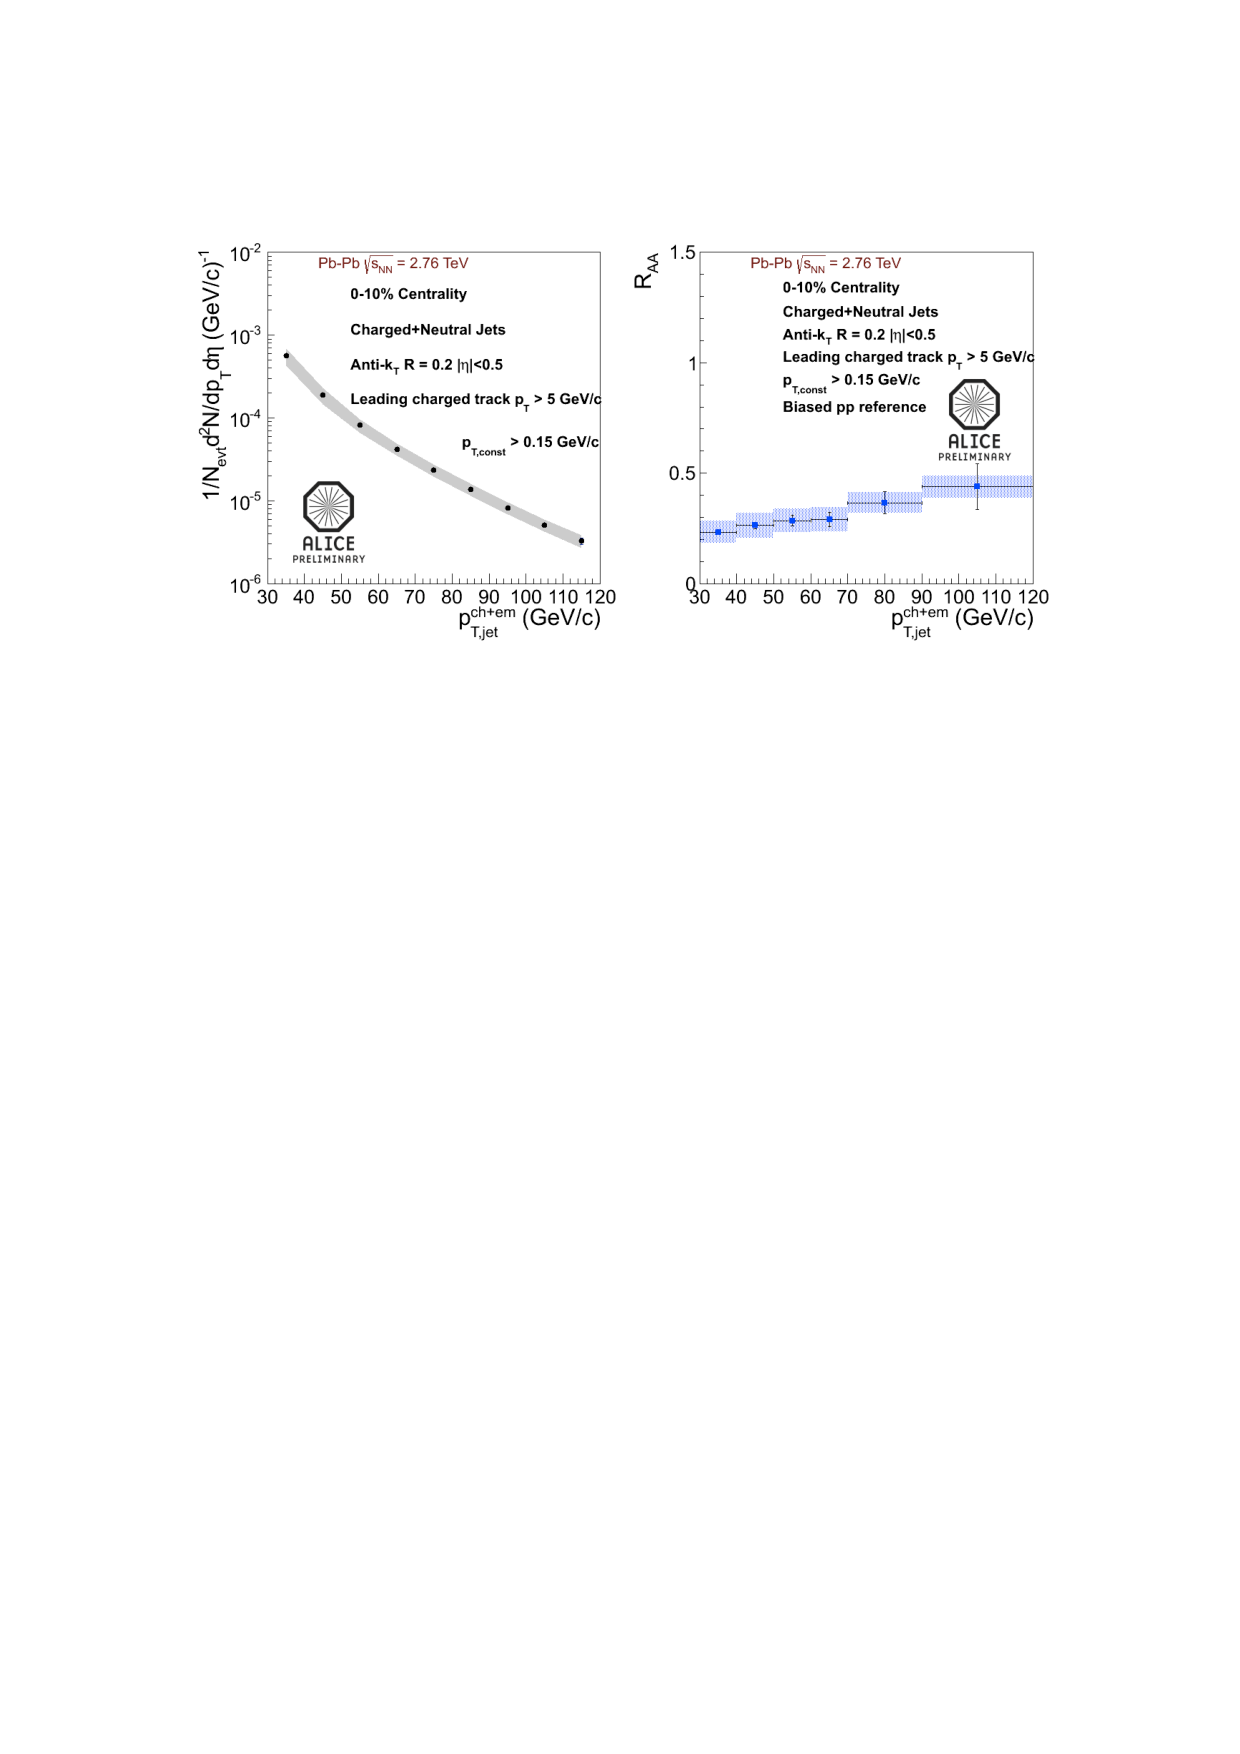
\includegraphics[width=0.85\textwidth]{figures/jetMeasurements/jet_raa_alice}
\caption{(Left) The inclusive jet cross section as a function of jet \pt\ in 0--10\% central \pbpb\ collisions at $\sqrtsnn = 2.76$ TeV.
The band around the data points represents the systematic uncertainty.
(Right) The \RAA\ for 0--10\% central \pbpb\ collisions.
Figure from Ref.~\cite{Reed_2013}.}
\label{fig:jet_raa_alice}
\end{center}
\end{figure}


These observations are consistent with results from ATLAS and CMS \cite{Aad:2014bxa, 2019108, Khachatryan:2016jfl, Verweij:2012ch}.
The ATLAS results at $\sqrtsnn = 5.02$ TeV are shown in Figure~\ref{fig:jetraa_atlas}.
The higher collision energy allows access to higher \pt\ jets.
The smooth centrality dependence can be more clearly seen in Figure~\ref{fig:raa_centDep_atlas}, where \RAA\ is shown as a function of \ANpart\ for jets the \mbox{100--126 GeV} and \mbox{200--251 GeV} ranges.
The magnitude of the suppression is also seen to significantly depend on jet \pt\ for $\ANpart \geq 50$.


%This measurement was conducted for jets in the 40--1000 GeV range in different rapidity and centrality intervals.
%The jet yields in \pp\ and \pbpb\ collisions are shown in Figure~\ref{fig:jet_yields} .
%The \pbpb\ jet yields are scaled by the thickness function and are shown for 8 centrality intervals.
%\begin{figure}[htbp]
%\begin{center}
%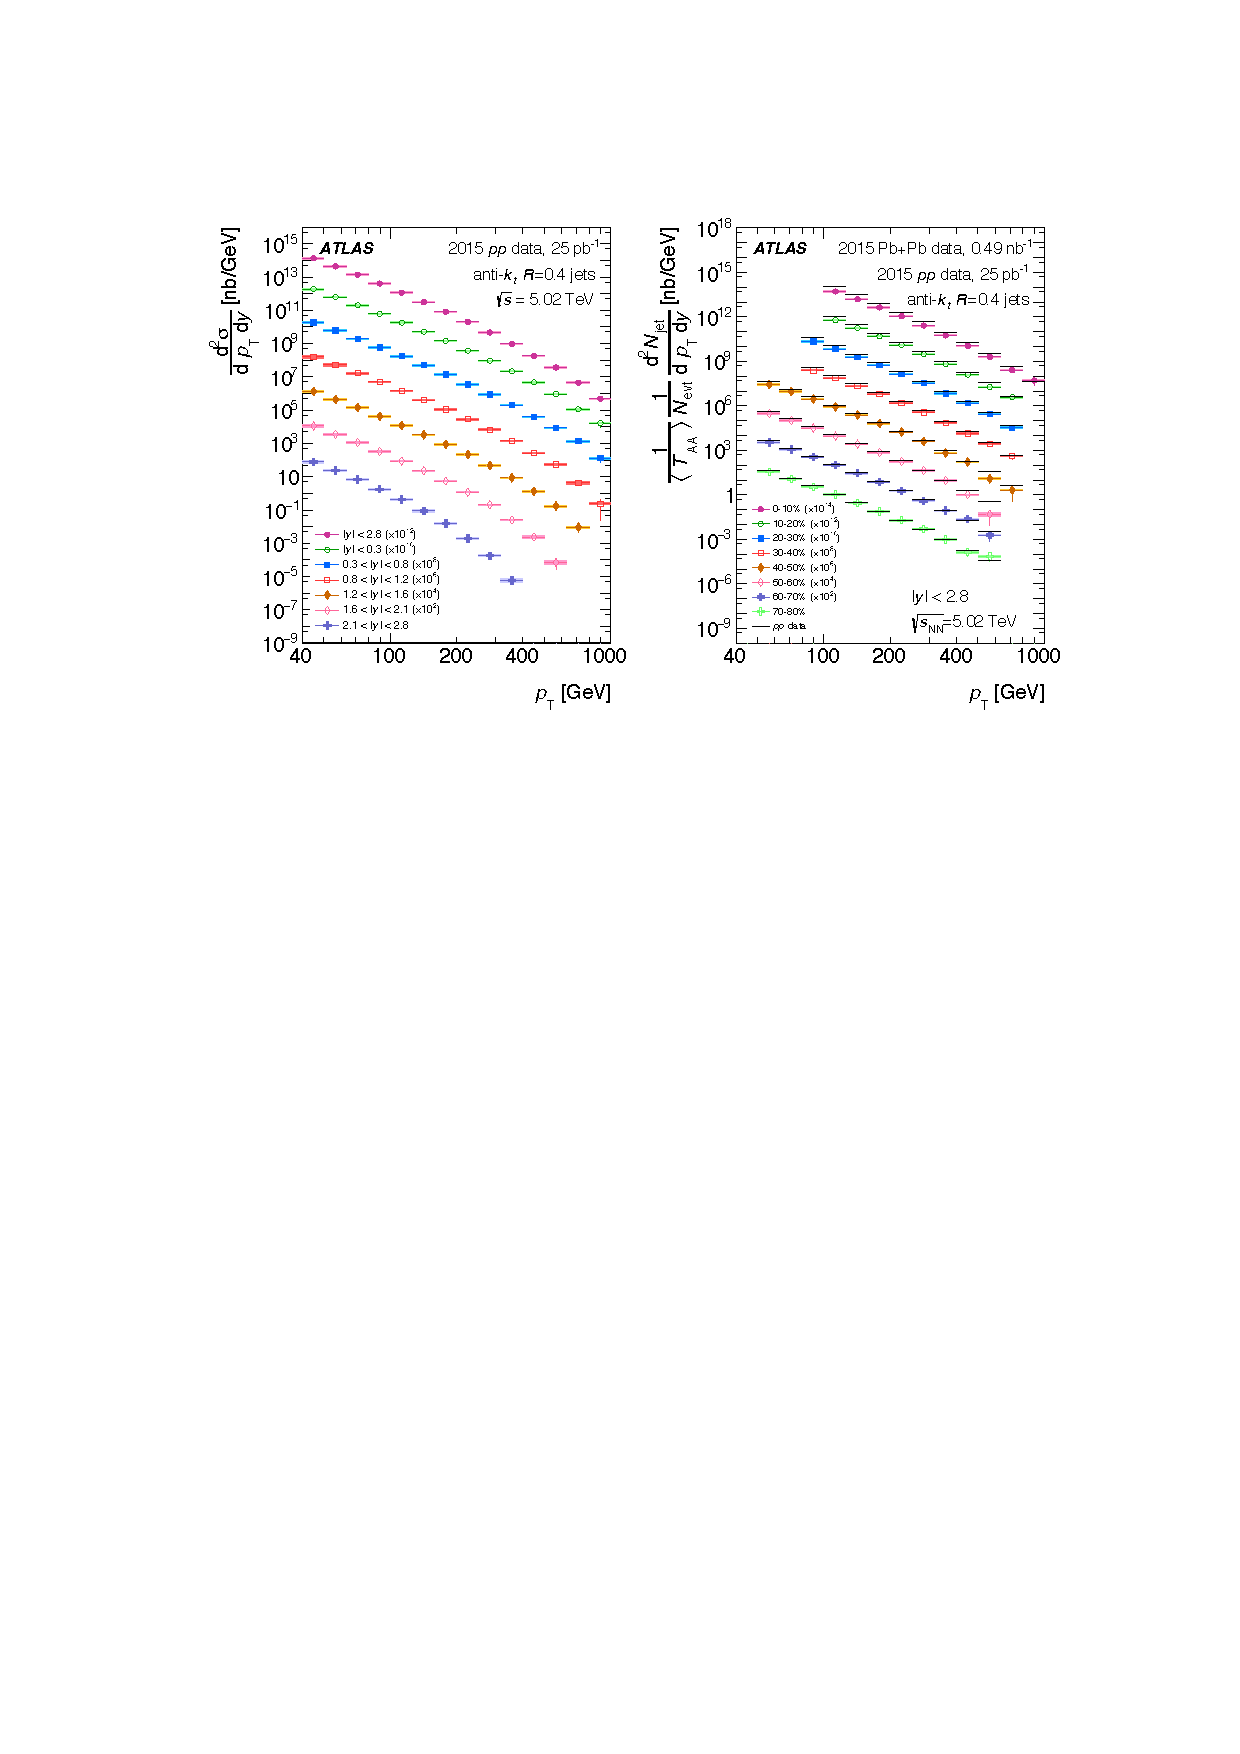
\includegraphics[width=0.85\textwidth]{figures/jetMeasurements/jetYields}
%\caption{(Left) The inclusive jet cross section in \pp\ collisions as a function of jet \pt\ in different $|y|$ intervals scaled by successive powers of $10^2$ for visibility.
%(Right) Per event inclusive jet yield in \pbpb\ collisions normalized by $\langle \TAA \rangle$ as a function of jet \pt\ in different centrality intervals scaled by successive powers of $10^2$ for visibility.
%The solid lines represent the cross section from \pp\ data at the same rapidity interval scaled by the same $10^2$ factor.
% Figure taken from Ref.~\cite{2019108}.}
%\label{fig:jet_yields}
%\end{center}
%\end{figure}
%Figure~\ref{fig:raa} shows the measured inclusive jet \RAA\ as a function of jet \pt\ for different centrality bins and jet rapidity $|y| < 2.8$.
%It can be seen that the most central collisions show a clear suppression with an $\RAA \approx 0.45$ at jet $\pt\ 100$ GeV.
%The \RAA\ value slowly evolves with jet \pt\ and rises to 0.6 at jet $\pt = 800$ GeV.
%This modification becomes smaller for more peripheral collisions.




\begin{figure}
\begin{subfigure}{.45\textwidth}
  \centering
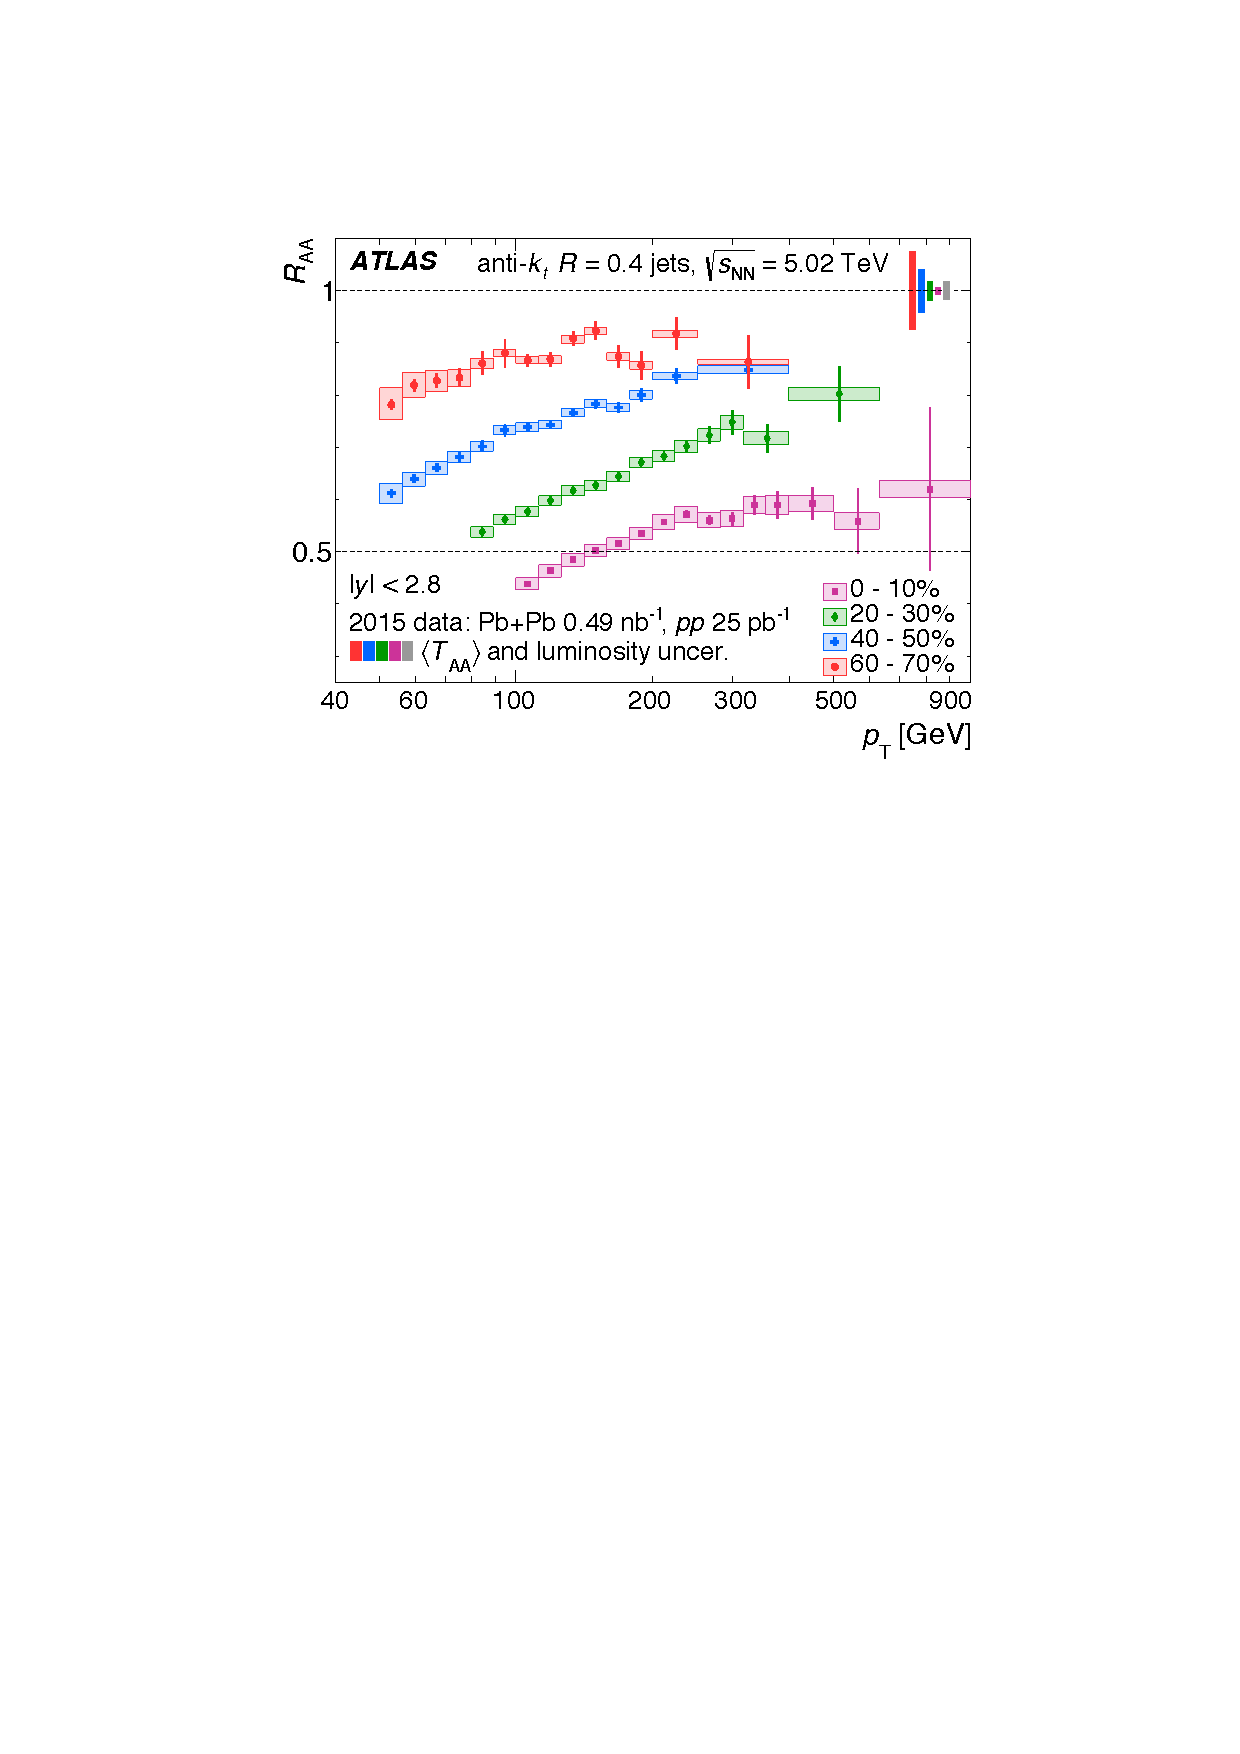
\includegraphics[width=\textwidth]{figures/jetMeasurements/raa}
\caption{}
\label{fig:jetraa_atlas}
\end{subfigure} \qquad
\begin{subfigure}{.45\textwidth}
  \centering
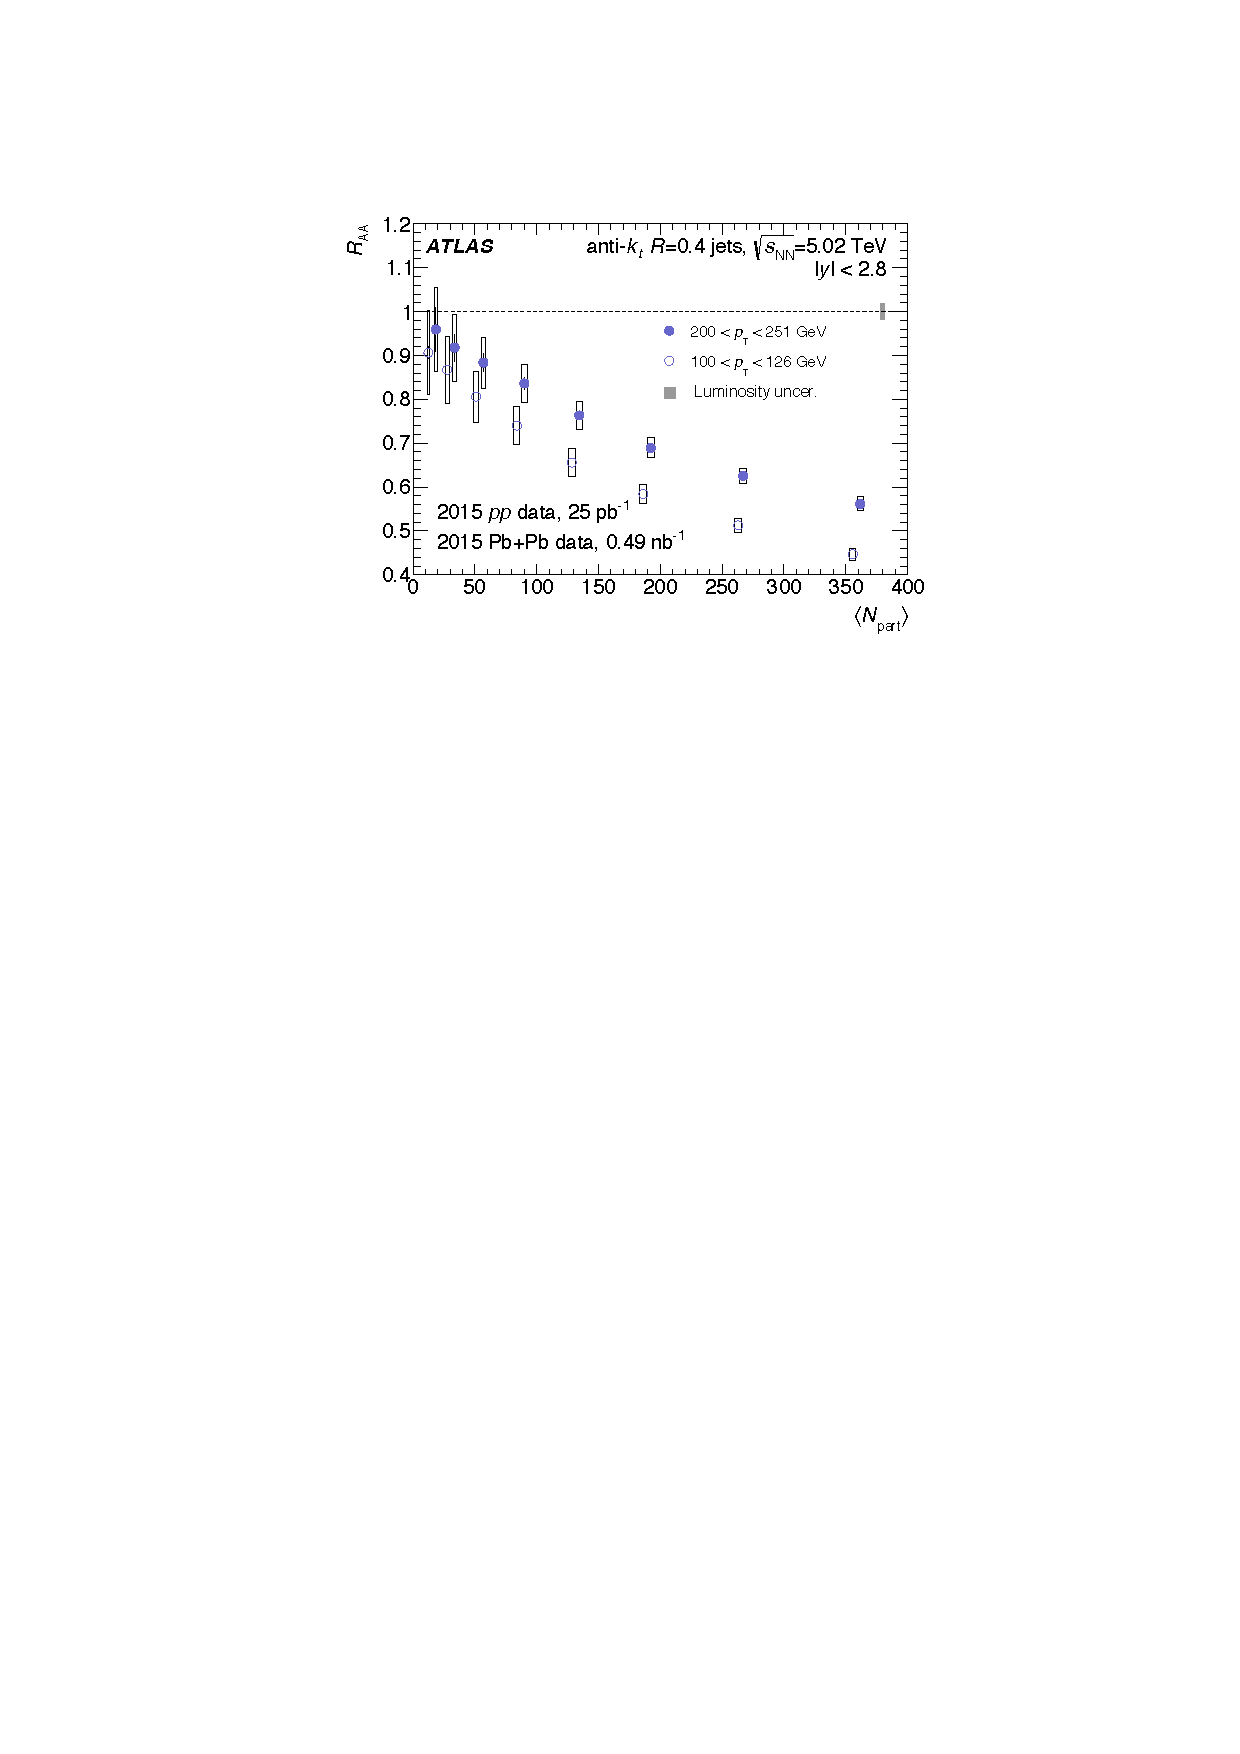
\includegraphics[width=\textwidth]{figures/jetMeasurements/raa_centDep}
\caption{}
\label{fig:raa_centDep_atlas}
\end{subfigure}
\caption{The \RAA\ distributions as a function of (left) jet \pt\ for different centrality bins and (right) $\langle \Npart \rangle$ for different jet \pt\ bins, for jet rapidity $|y| < 2.8$.
Figures from Ref.~\cite{2019108}.}
\label{fig:atlas_jet_raa}
\end{figure}

%
%\begin{figure}
%\begin{center}
%  \begin{minipage}[b]{0.43\textwidth}
%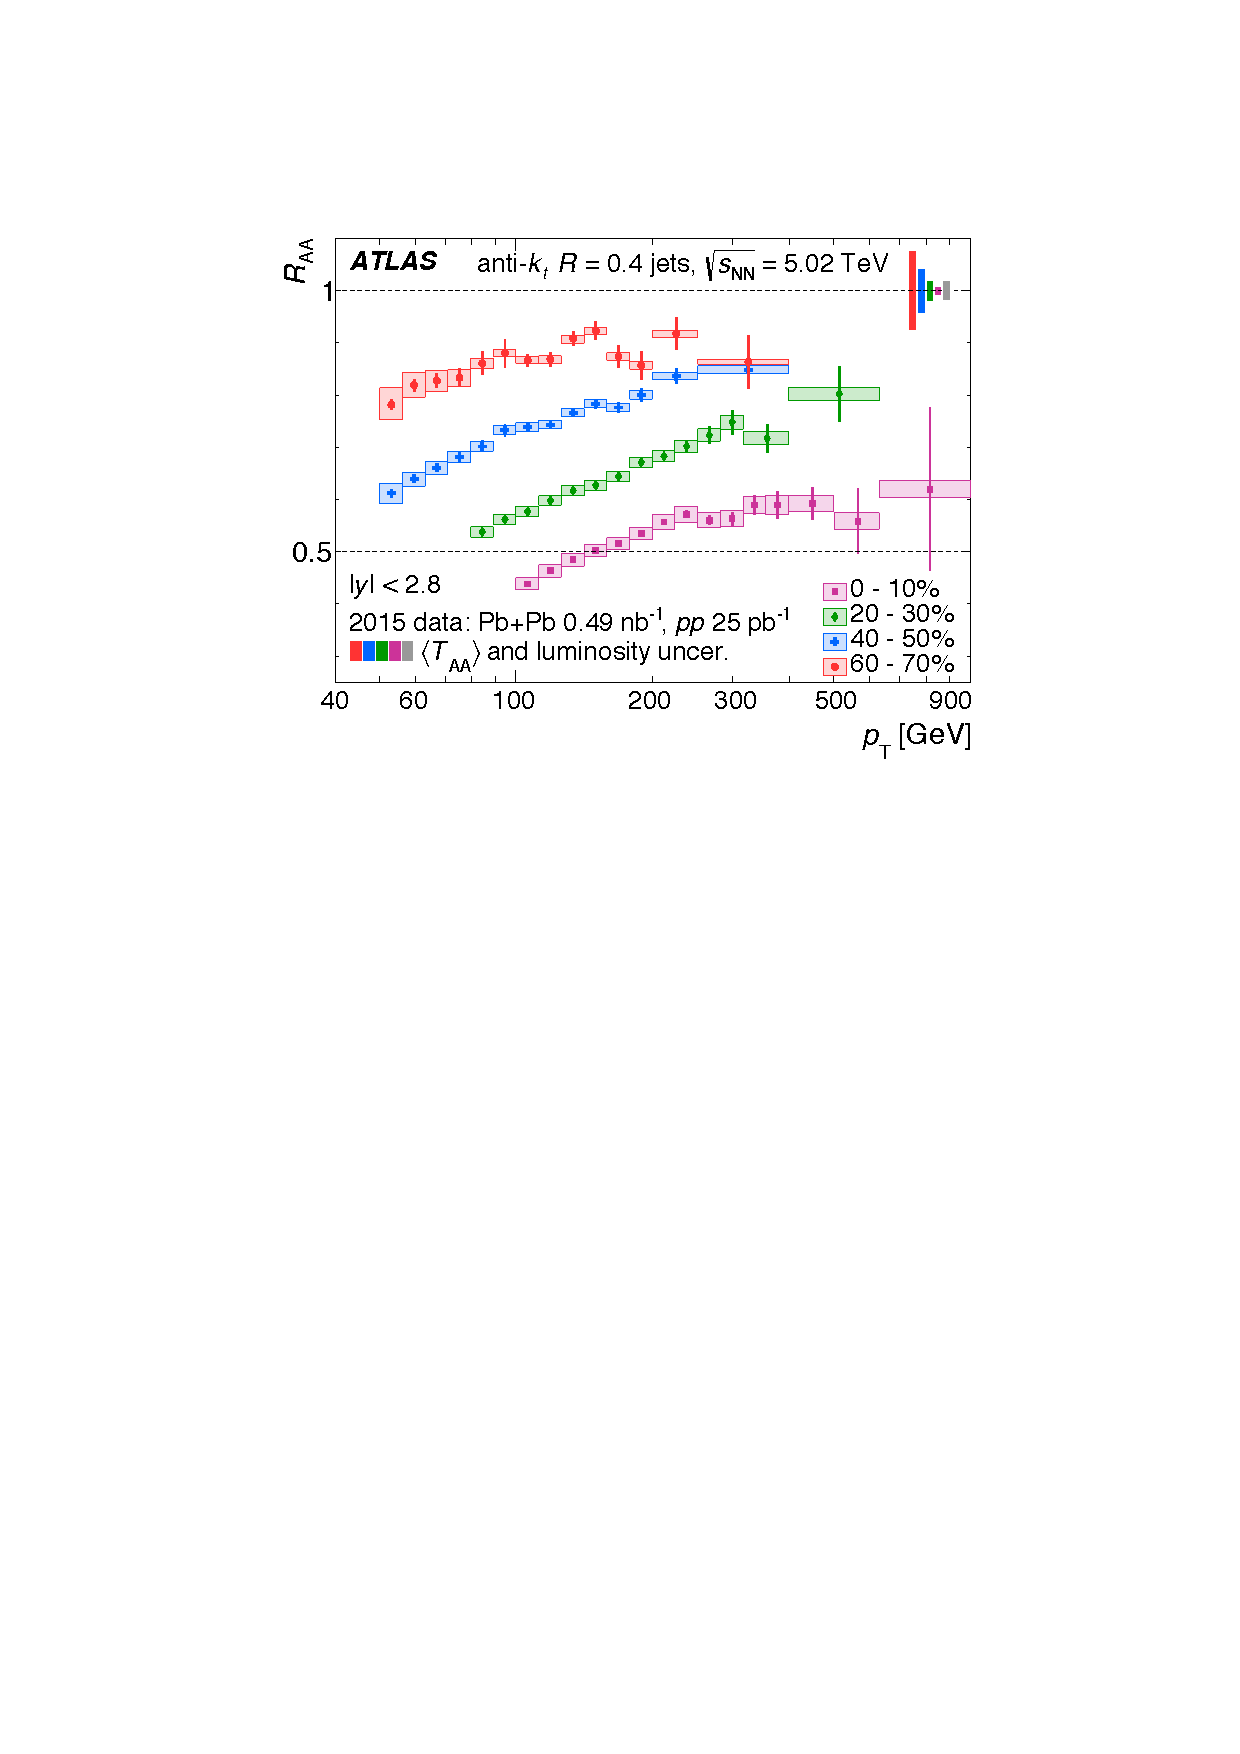
\includegraphics[width=\textwidth]{figures/jetMeasurements/raa}
%\caption{The \RAA\ distributions as a function of jet \pt\ for different centrality bins and jet rapidity $|y| < 2.8$.
%The error bars represent statistical uncertainties while the shaded boxes represent systematic uncertainties.
%Figure taken from Ref.~\cite{2019108}.}
%\label{fig:raa}
%  \end{minipage}
% \qquad  \qquad  \qquad
%  \begin{minipage}[b]{0.43\textwidth}
%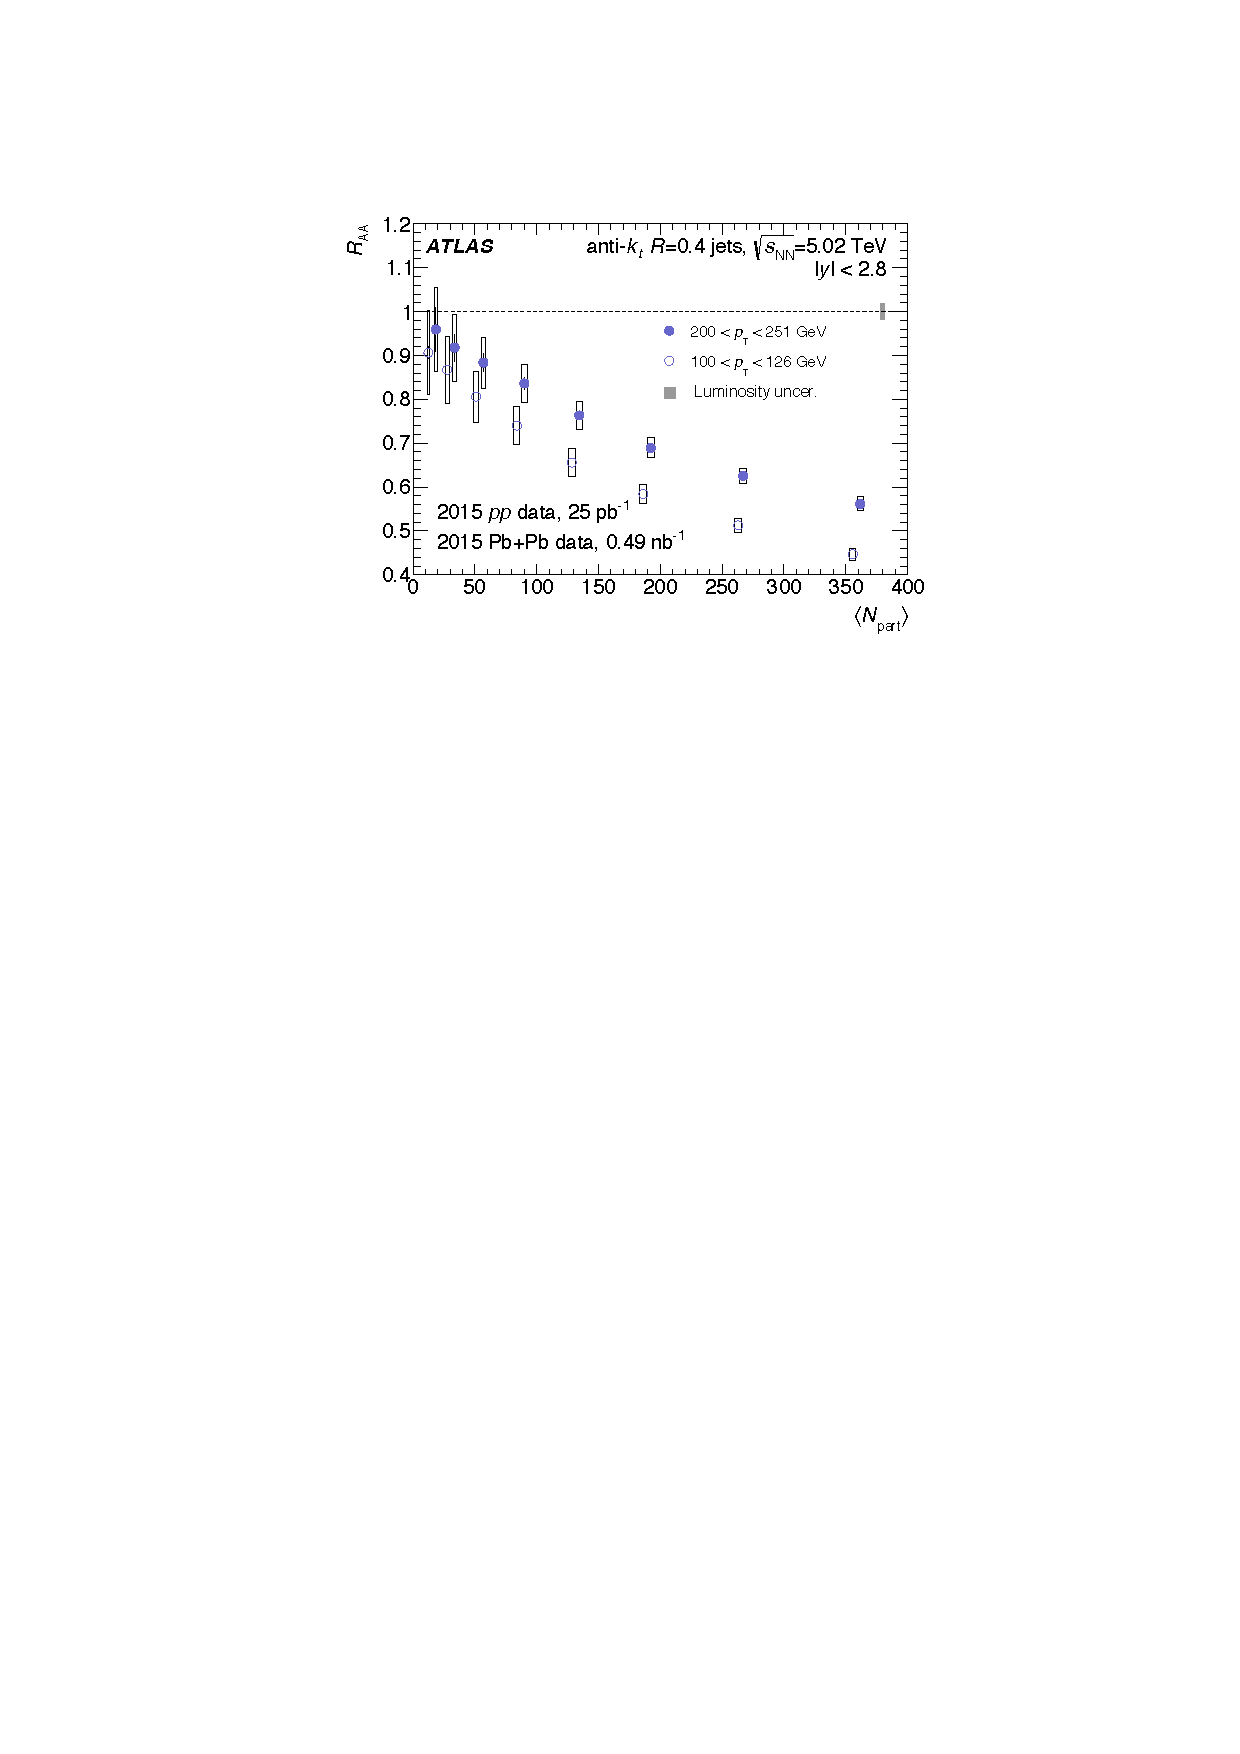
\includegraphics[width=\textwidth]{figures/jetMeasurements/raa_centDep}
%\caption{The \RAA\ distributions as a function of jet \pt\ for different centrality bins and jet rapidity $|y| < 2.8$.
%The error bars represent statistical uncertainties while the shaded boxes represent systematic uncertainties.
%Figure taken from Ref.~\cite{2019108}.}
%\label{fig:raa_centDep}
%  \end{minipage}
%  \end{center}
%\end{figure}

%
%\begin{figure}[htbp]
%\begin{center}
%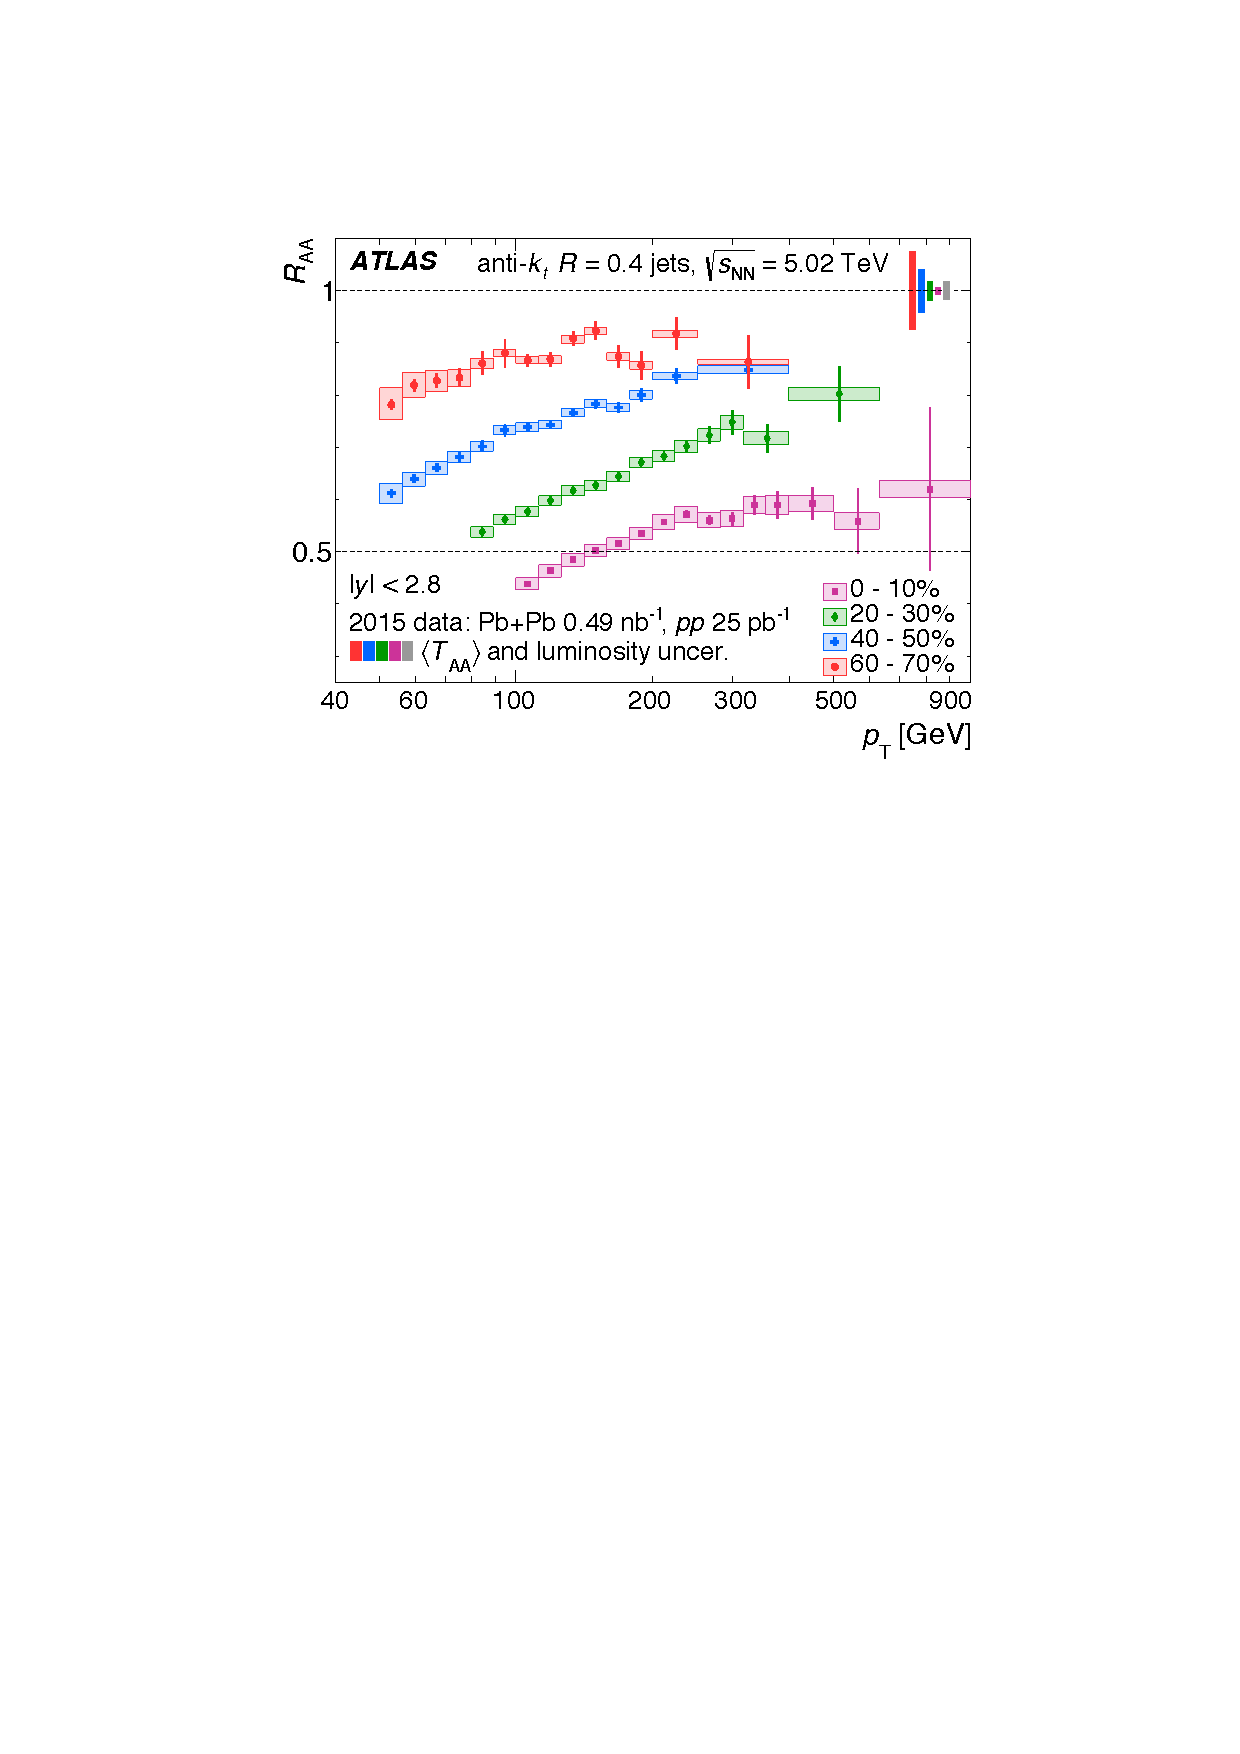
\includegraphics[width=0.55\textwidth]{figures/jetMeasurements/raa}
%\caption{The \RAA\ distributions as a function of jet \pt\ for different centrality bins and jet rapidity $|y| < 2.8$.
%The error bars represent statistical uncertainties while the shaded boxes represent systematic uncertainties.
%Figure taken from Ref.~\cite{2019108}.}
%\label{fig:raa}
%\end{center}
%\end{figure}


%\begin{figure}[htbp]
%\begin{center}
%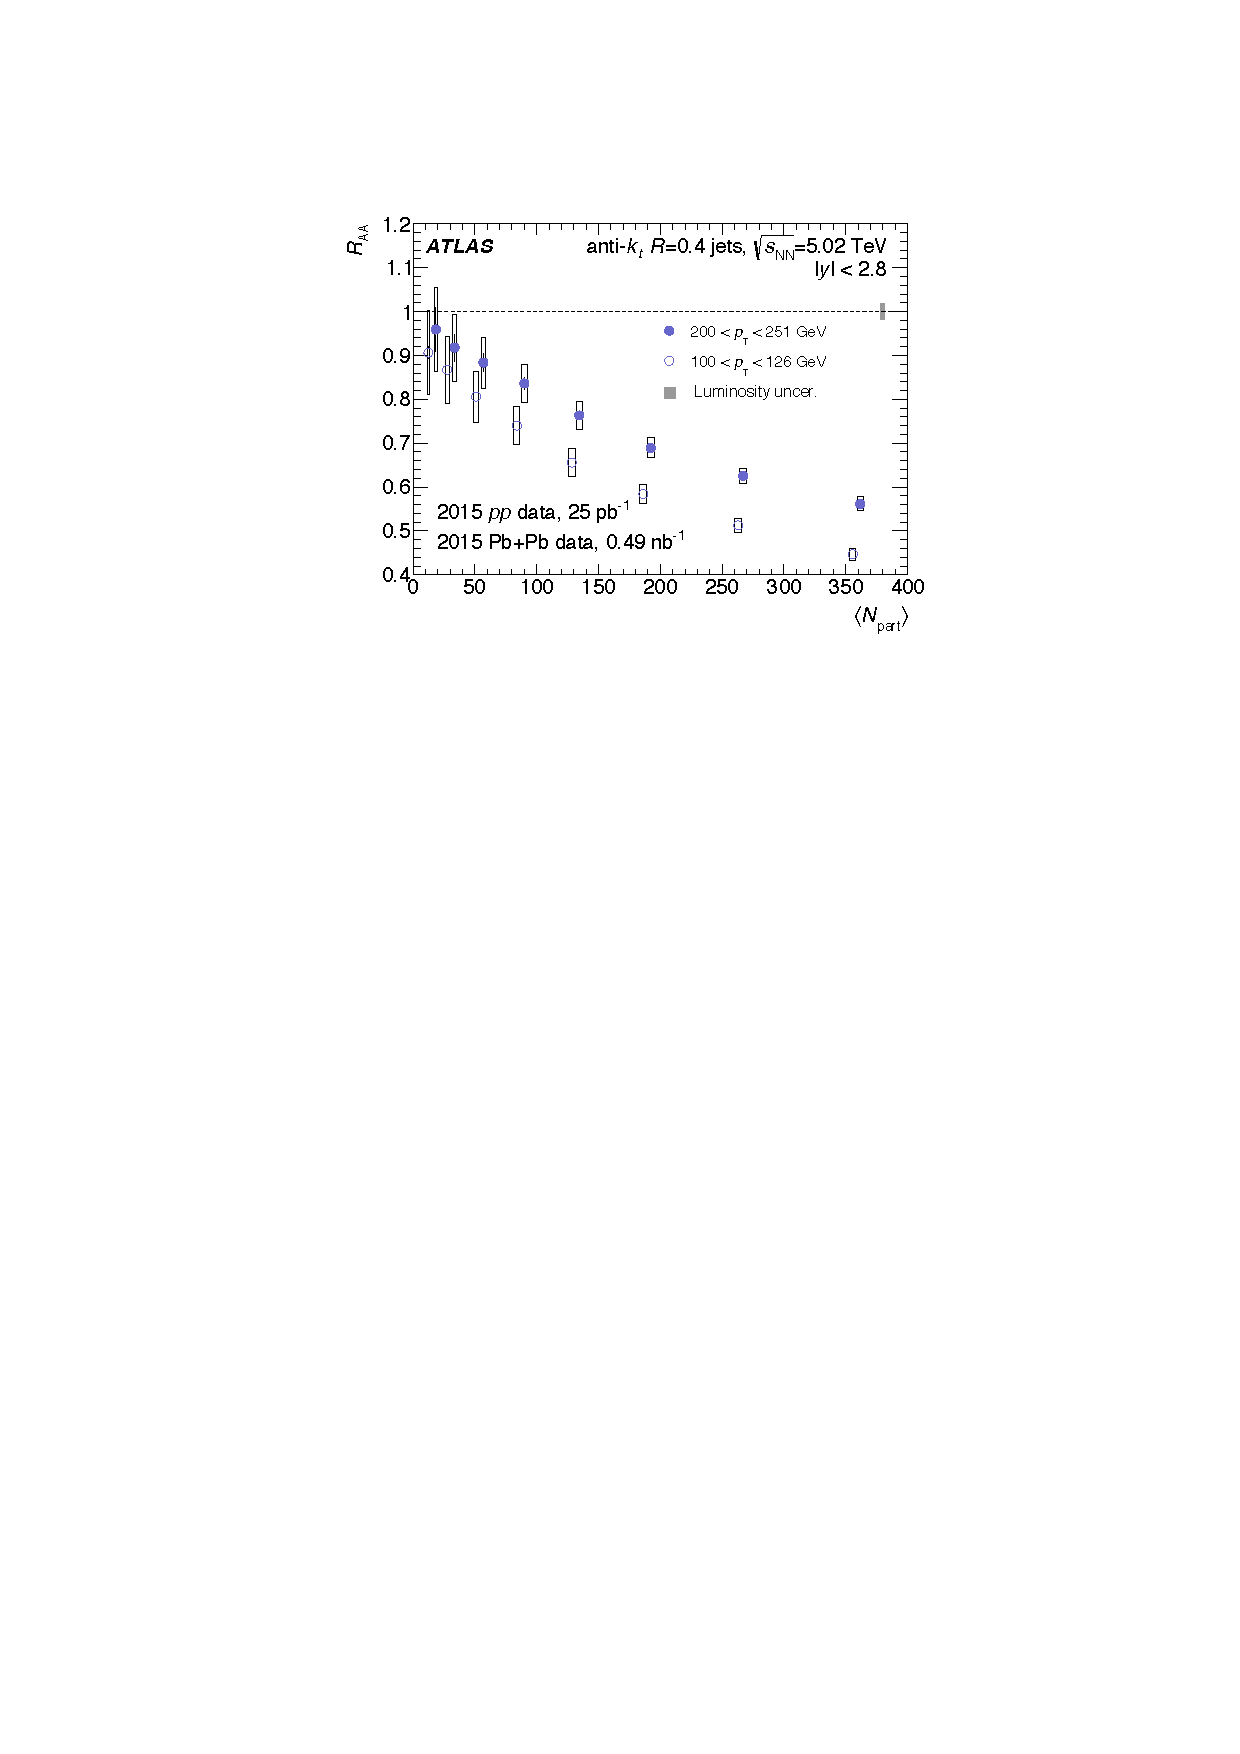
\includegraphics[width=0.55\textwidth]{figures/jetMeasurements/raa_centDep}
%\caption{The \RAA\ distributions as a function of jet \pt\ for different centrality bins and jet rapidity $|y| < 2.8$.
%The error bars represent statistical uncertainties while the shaded boxes represent systematic uncertainties.
%Figure taken from Ref.~\cite{2019108}.}
%\label{fig:raa_centDep}
%\end{center}
%\end{figure}

%The measurement further looked at the $y$ dependence of \RAA\ as described by $\RAA (|y|) / \RAA (|y| < 0.3)$.
%This is useful because it is sensitive to the different quark to gluon fractions at different rapidities.
% the uncertainties largely cancel, an





\section{Jet Fragmentation}
\label{sec:jet_ff}
% !TEX encoding = UTF-8 Unicode
% !TEX root = thesis-ex.tex

This section will discuss the jet fragmentation as measured by the ATLAS detector for \pbpb\ collisions at $\sqrtsnn = 5.02$ TeV \cite{PhysRevC.98.024908}.
While measurements of \RAA \cite{20151, Aad:2014bxa, Khachatryan:2016jfl} and asymmetry \cite{Aaboud:2017eww, Chatrchyan:2011sx, PhysRevLett.119.062301} describe how much energy is lost by the jet, fragmentation measurements describe the momentum distribution of particles associated to the jet.
These can be described as:

\begin{align}
\Dz = \frac{1}{\Njet} \frac{d\nch}{dz} \\
\Dpt = \frac{1}{\Njet} \frac{d\nch}{d\pt}
\end{align}
where $z = \pt \cos(\Delta R / \ptjet)$ and gives the charged-particle longitudinal momentum fraction relative to the jet.
Modifications to the fragmentation functions in \pbpb\ collisions can be evaluated by constructing the ratios $\Rdz = \Dz_{\rm Pb+Pb} / \Dz_{pp}$ and $\Rdpt = \Dpt_{\rm Pb+Pb} / \Dpt_{pp}$.
This measurement is corrected for detector effects and unfolded to the particle level.
This allows for comparisons to other measurements and theoretical models.
The \Dpt\ distribution is shown in Figure~\ref{fig:jetff_dpt}.

\begin{figure}[htbp]
\begin{center}
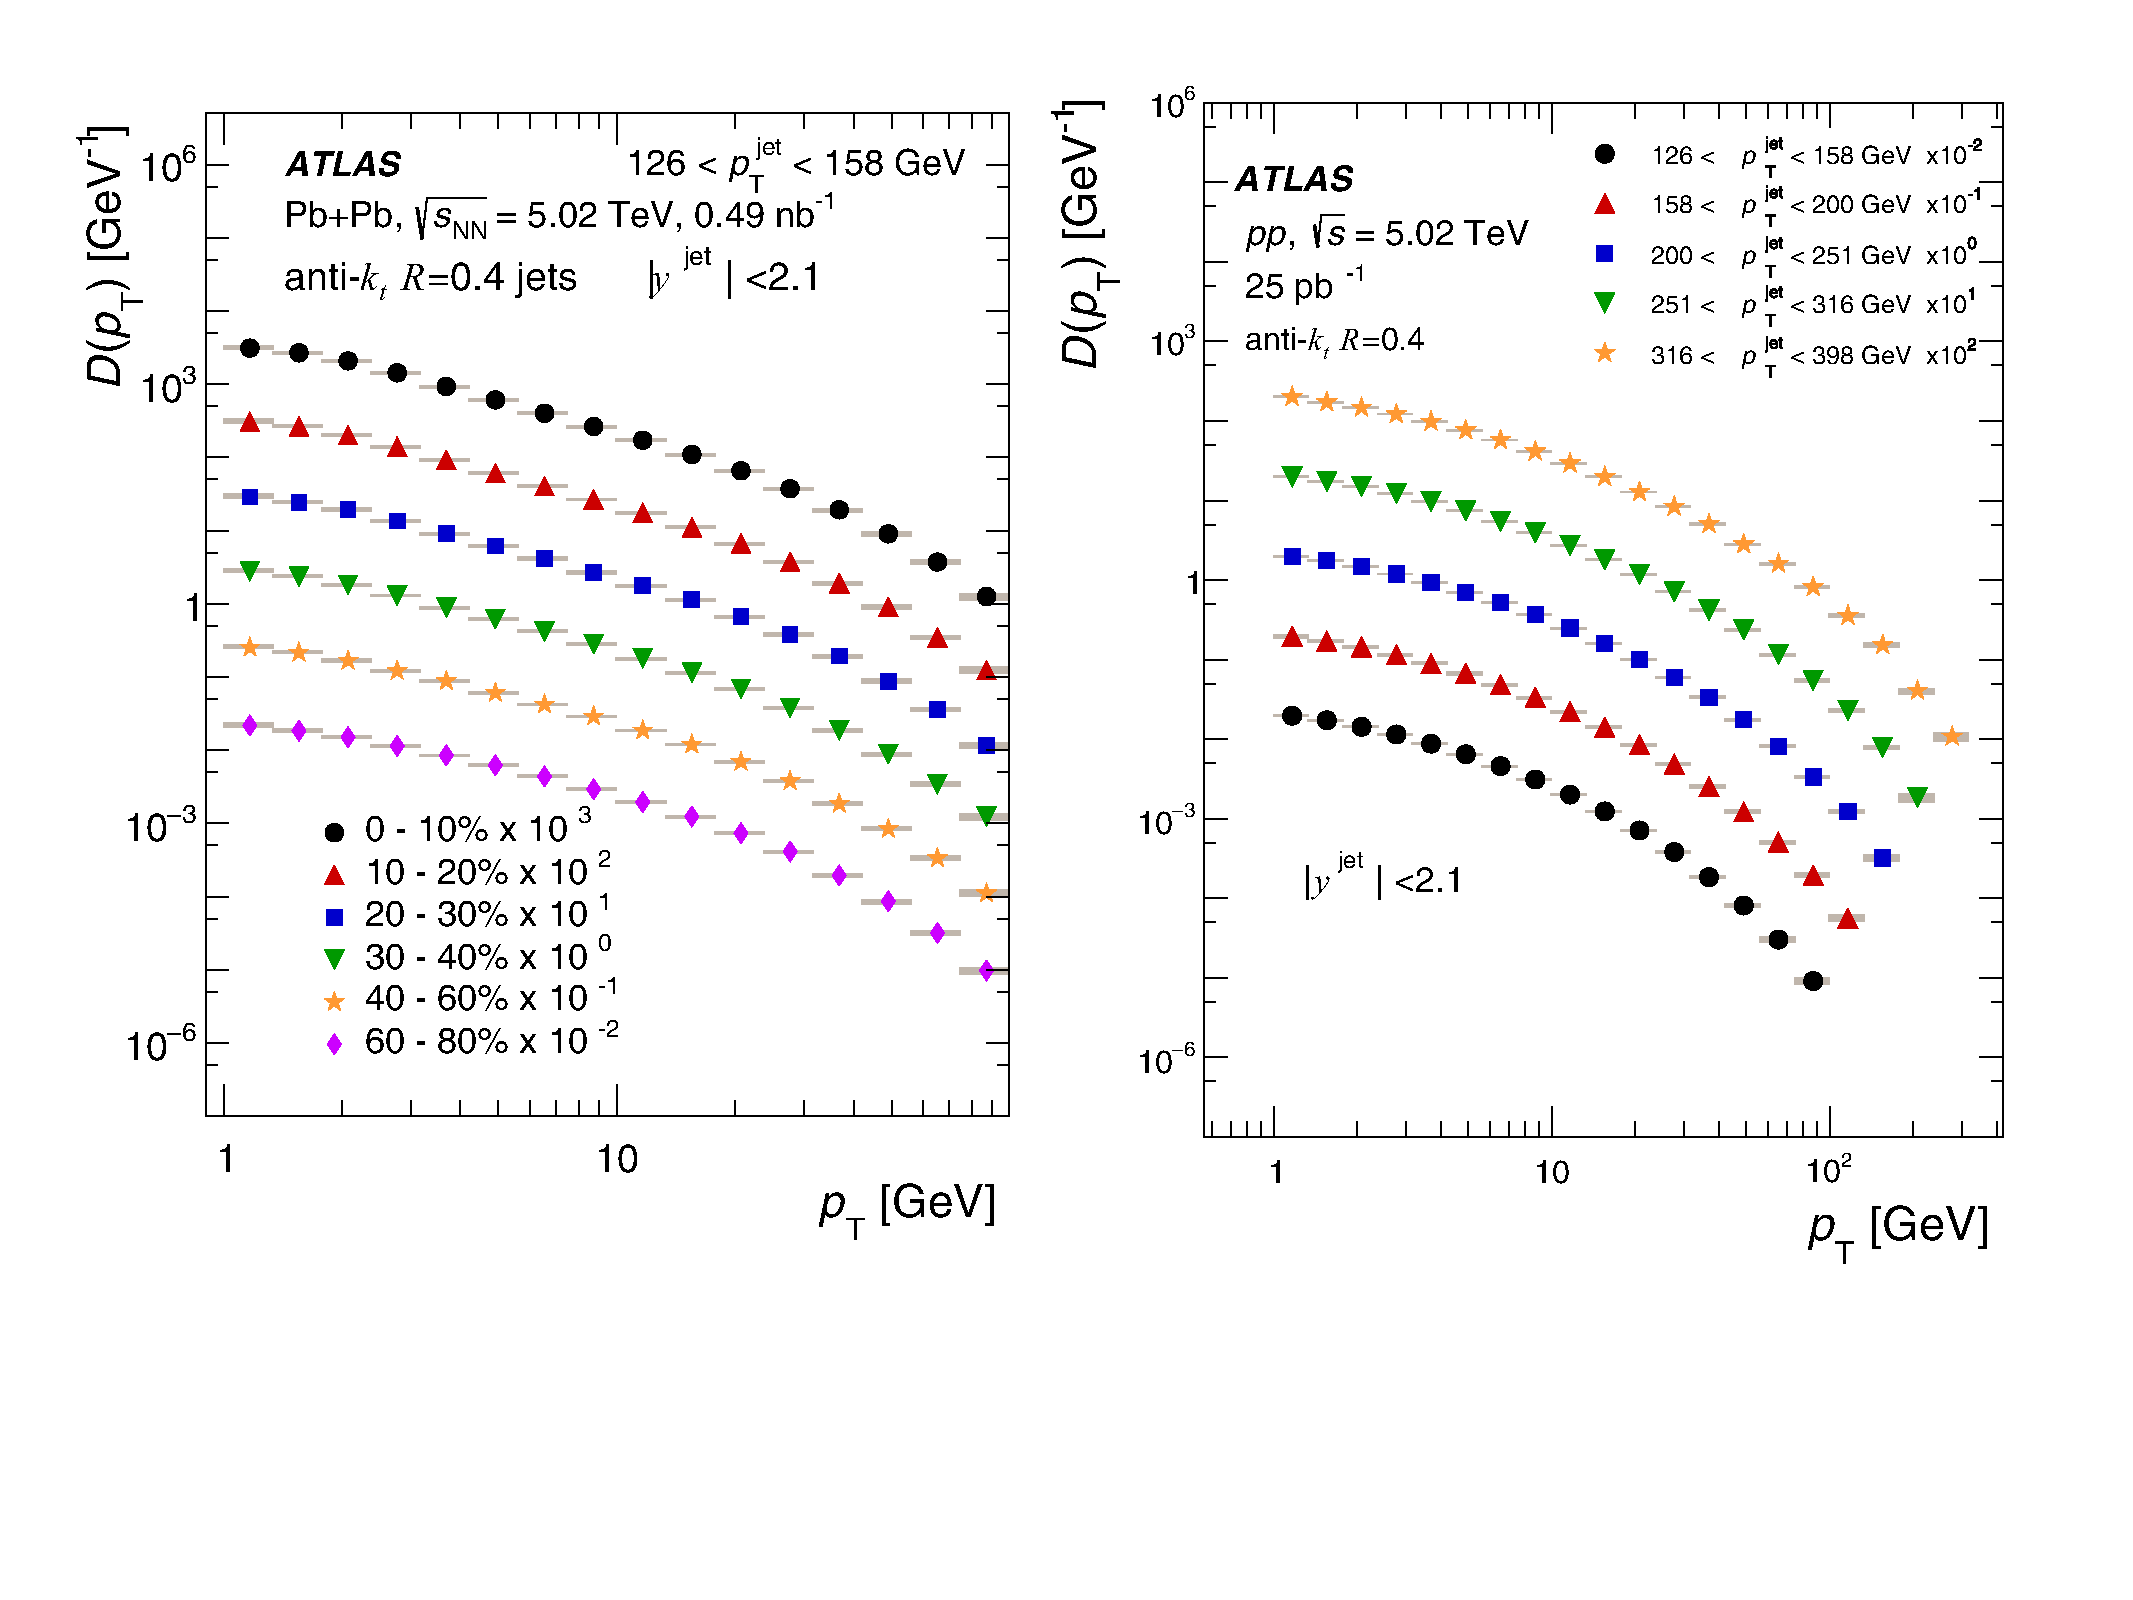
\includegraphics[width=0.65\textwidth]{figures/jetMeasurements/jetff_dpt}
\caption{(Left) The \Dpt\ distributions in \pp\ as a function of charged-particle \pt\ for different \ptjet\ selections and for jet rapidity $|y| < 2.1$.
(Right) The \Dpt\ distributions in \pbpb\ as a function of charged-particle \pt\ for different centrality selections and for jet rapidity $|y| < 2.1$.
The error bars represent statistical uncertainties while the shaded boxes represent systematic uncertainties.
Figure taken from \cite{PhysRevC.98.024908}.}
\label{fig:jetff_dpt}
\end{center}
\end{figure}


\begin{figure}[htbp]
\begin{center}
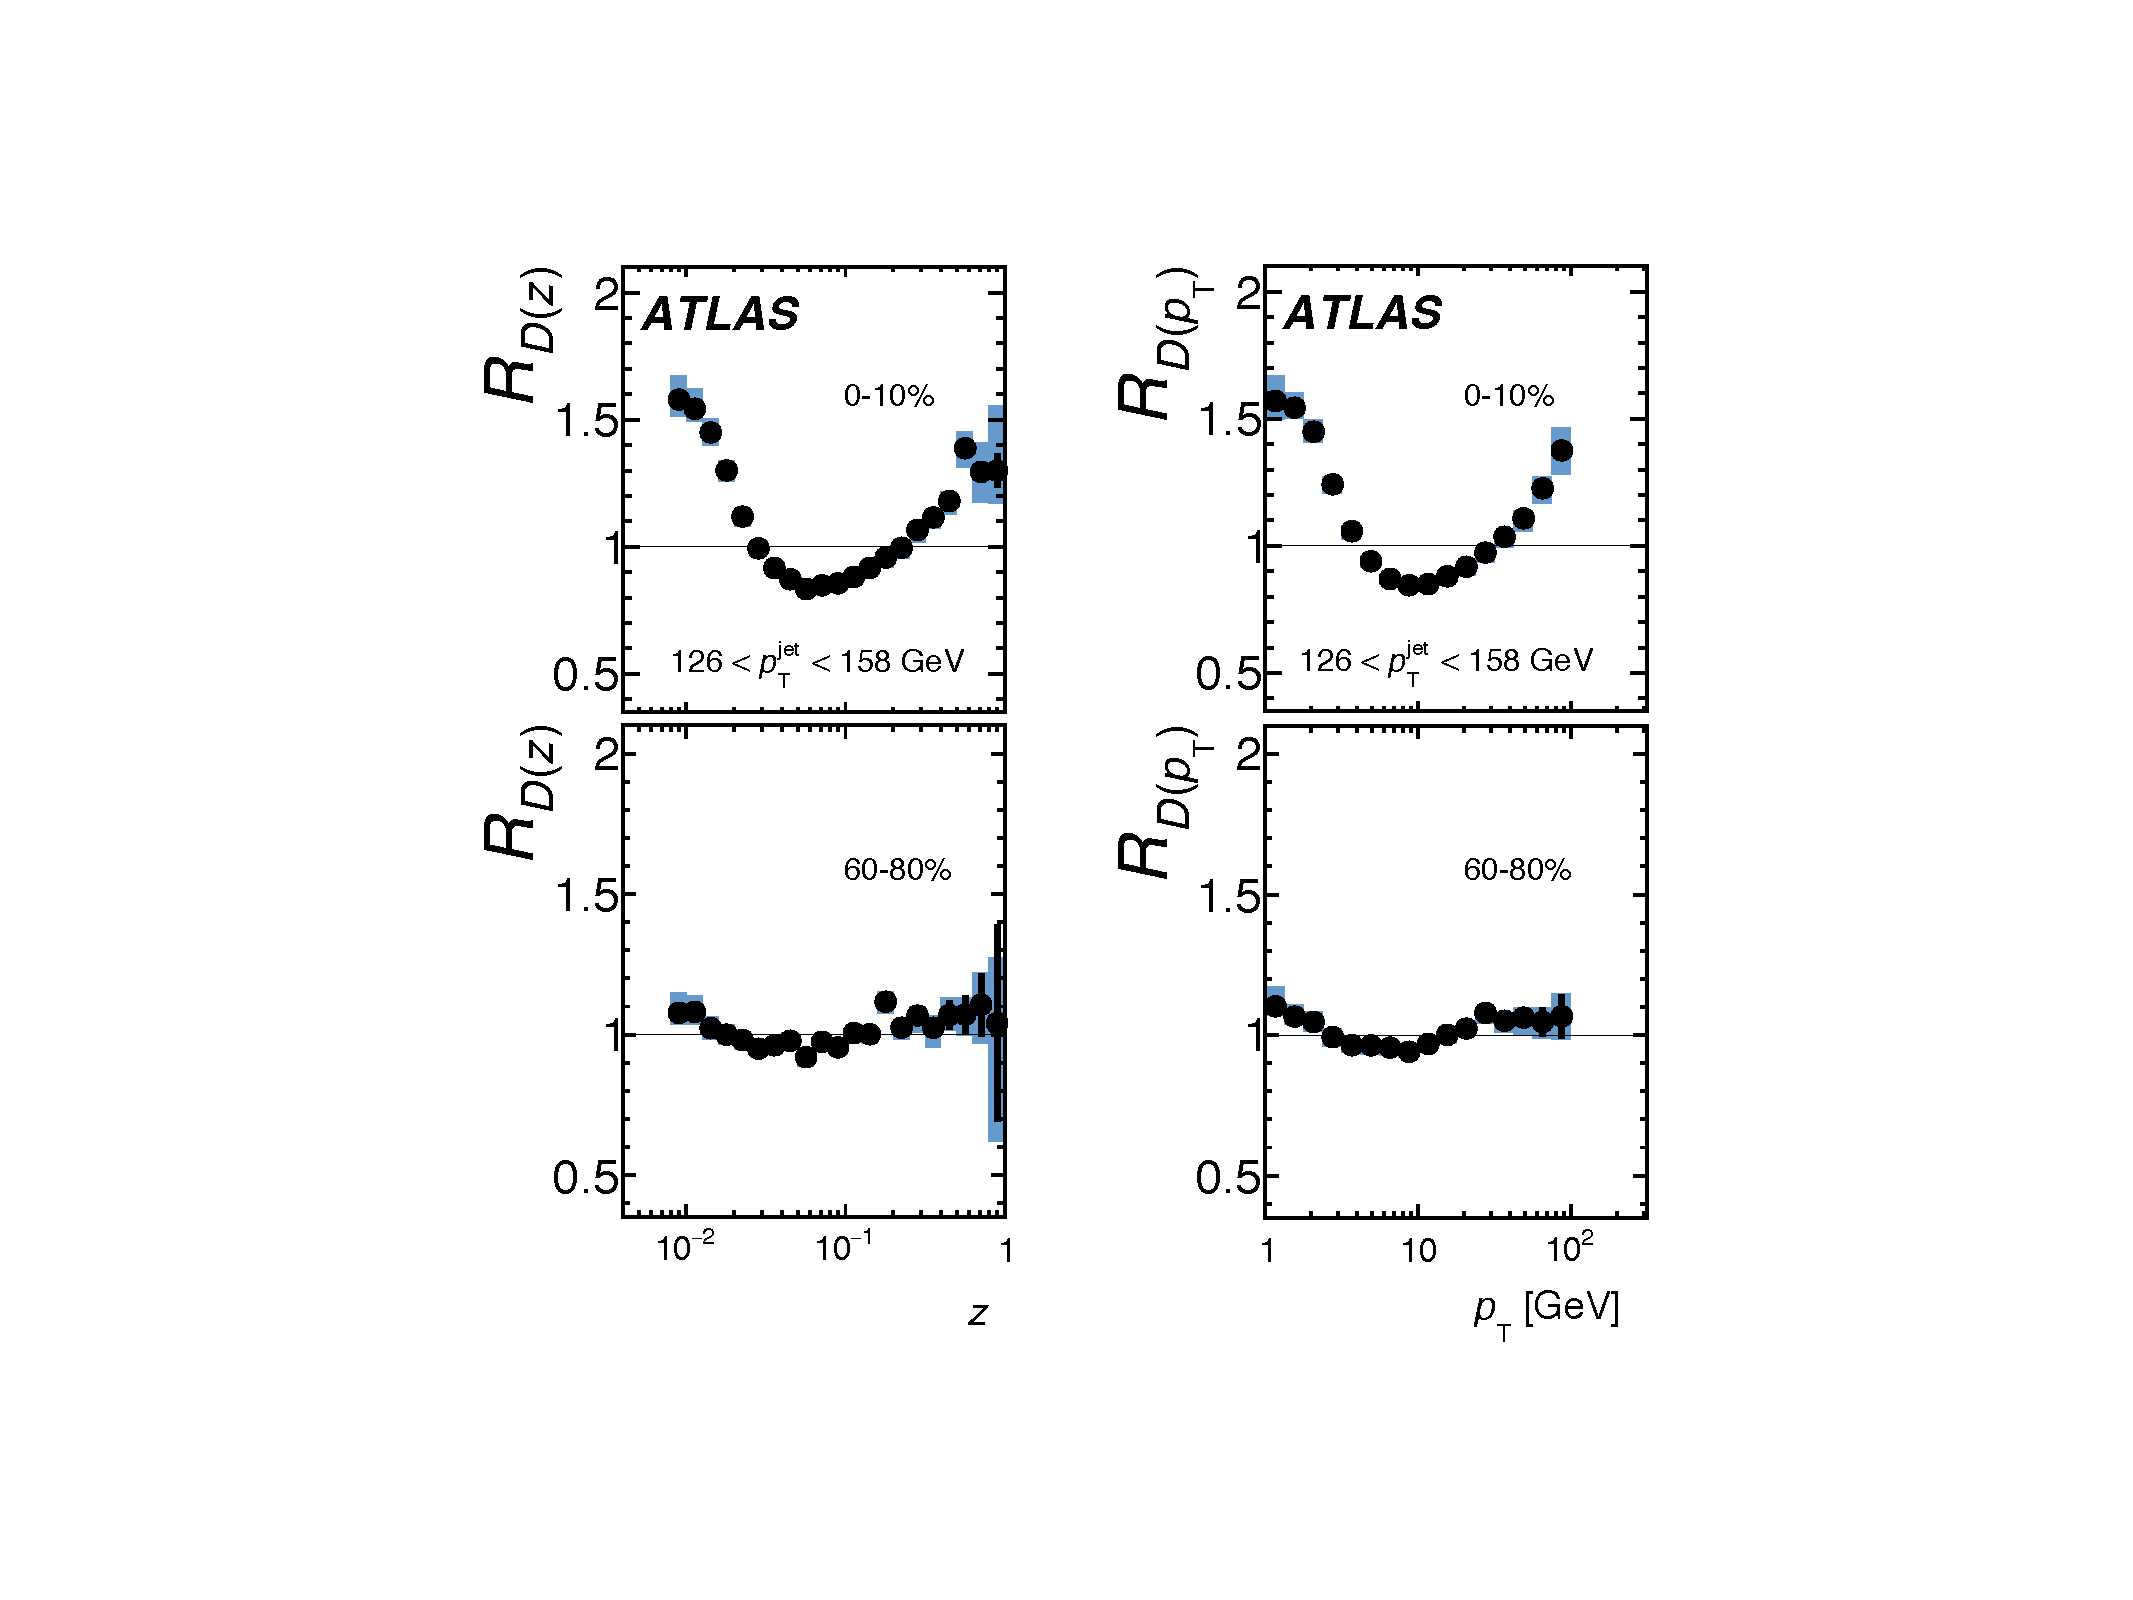
\includegraphics[width=0.65\textwidth]{figures/jetMeasurements/jetff_rdz_rdpt}
\caption{The modifications to the (left) \Dz\ and (right) \Dpt\ distributions in (top) 0--10\% central and (bottom) peripheral \pbpb\ compared to \pp\ as a function of charged-particle $z$ and \pt\ respectively.
The error bars represent statistical uncertainties while the shaded boxes represent systematic uncertainties.
Figures taken from \cite{PhysRevC.98.024908}.}
\label{fig:jetff_rdz_rdpt}
\end{center}
\end{figure}

The modifications to the \Dz\ and \Dpt\ distributions in central (top) and peripheral (bottom) collisions are shown in Figure~\ref{fig:jetff_rdz_rdpt}.
The shape of these modifications is very similar for both \Dz\ and \Dpt.
There is an enhancement of particles with low $z$ and \pt, followed by a suppression at intermediate $z$ and \pt, and finally an enhancement at high $z$ and \pt.
These modifications become smaller for more peripheral collisions.
The low momentum excess can be further investigated by calculating the extra number of particles \Nch\ in \pbpb\ compared to \pp\ as given below:

\begin{align}
\Nch = \int^{\pt_{\mathrm{max}}}_{\pt_{\mathrm{min}}} \left( \Dpt_{\pbpb} - \Dpt_{\pp} \right) d\pt
\end{align}
where $\pt_{\mathrm{min}} = 1$ GeV and $\pt_{\mathrm{max}} = 4.2$ GeV.

The \Nch\ distributions can be seen in Figure~\ref{fig:jetff_nch}.
It can be clearly seen that the size of the enhancement in \pp\ compared to \pp\ at low \pt\ increases as a function of \ptjet, growing from about 1.5 to 2.5 extra particles in the most central \pbpb\ collisions.
This excess is even seen in the peripheral \pbpb\ collisions, though it is a lot smaller and ranges from 0.2 to 0.5 extra particles.



%The \ptjet\ dependence of the \Rdz\ and \Rdpt\ distributions can be seen in Figure~\ref{fig:jetff_jetpt_dep}.
%This dependence can give insight into the modification of the fragmentation functions, with any scaling with $z$ indicating a change in the fragmentation pattern, while a scaling with \pt\ reflecting an effect from the medium itself.
%The low momentum excess in the \Rdpt\ distributions seen in Figure~\ref{fig:jetff_jetpt_dep} can be further studied by integrating over that region.
%Then the extra number of particles in \pbpb\ compared to \pp\ is given by:
%\begin{figure}[htbp]
%\begin{center}
%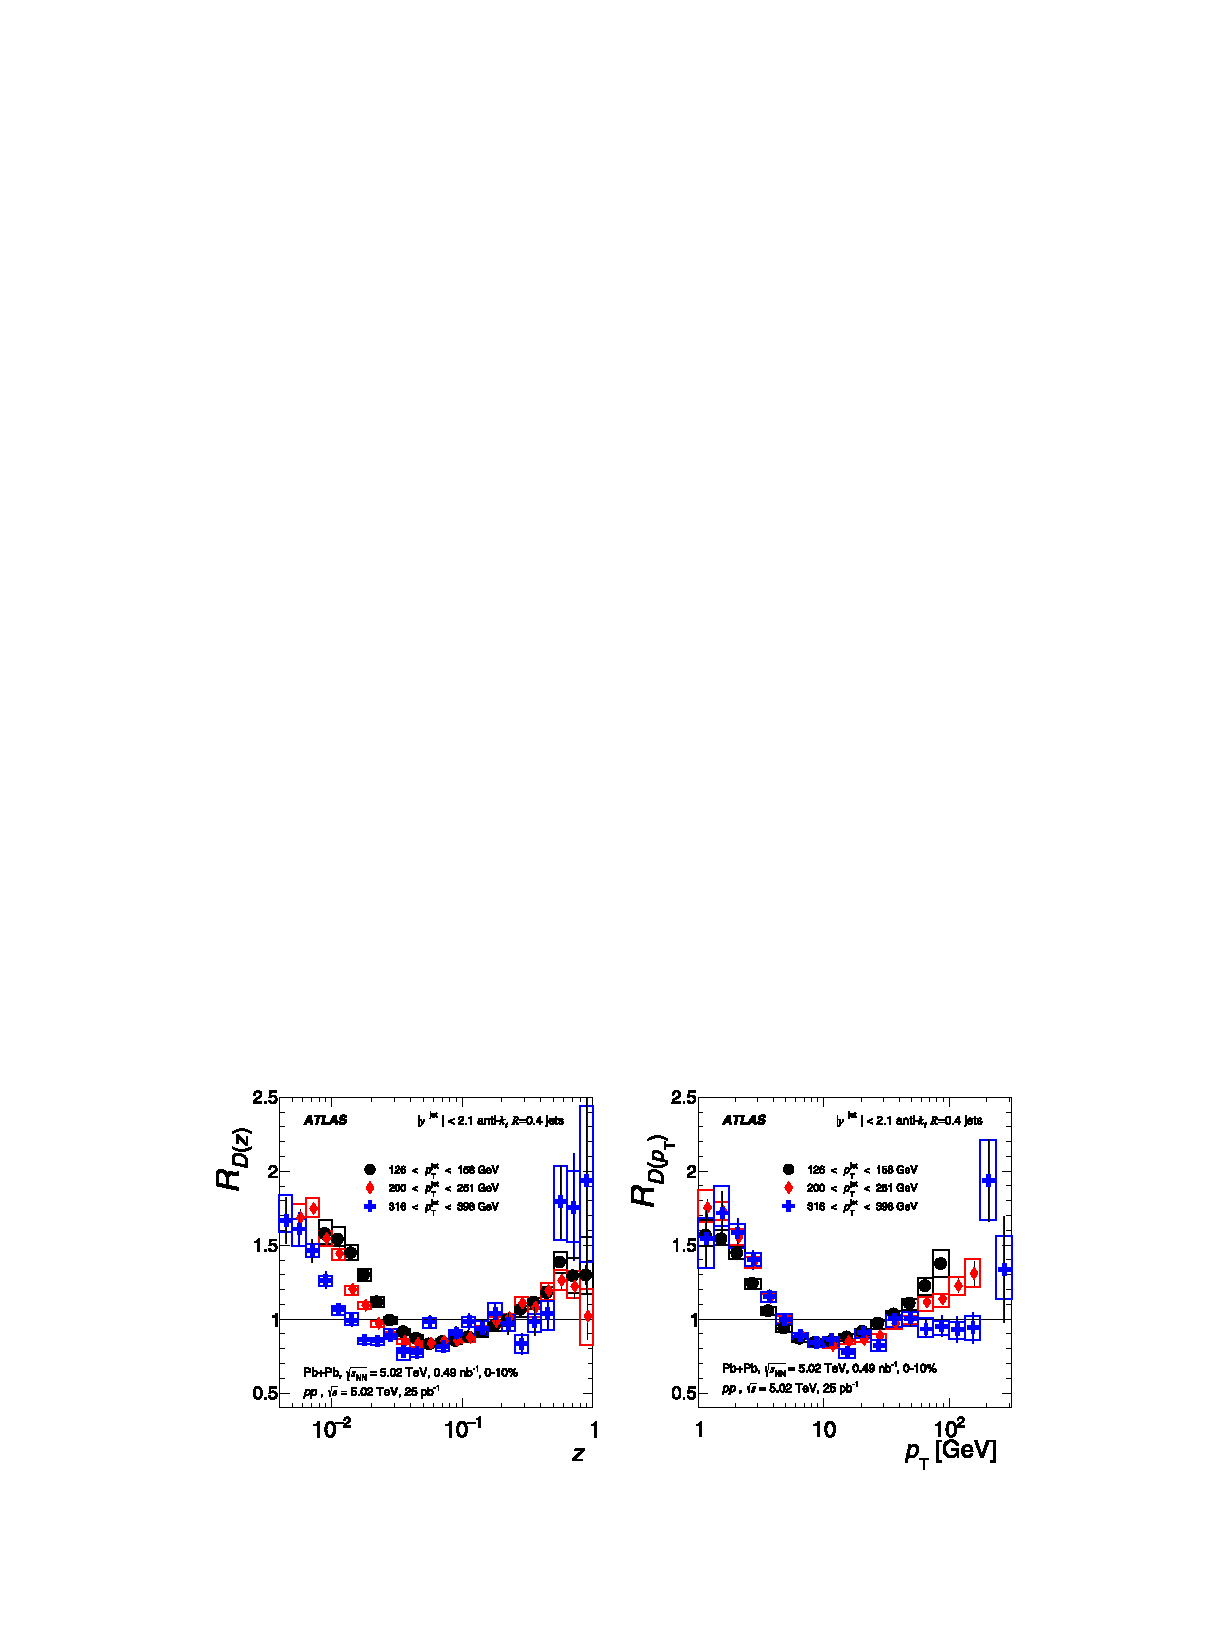
\includegraphics[width=0.75\textwidth]{figures/jetMeasurements/jetff_jetpt_dep}
%\caption{The \ptjet\ dependence of the \Rdz\ (left) and \Rdpt\ (right) distributions in 0--10\% central \pbpb\ compared to \pp\ collisions.
%The error bars represent statistical uncertainties while the shaded boxes represent systematic uncertainties.
%Figure taken from \cite{PhysRevC.98.024908}.}
%\label{fig:jetff_jetpt_dep}
%\end{center}
%\end{figure}


\begin{figure}[htbp]
\begin{center}
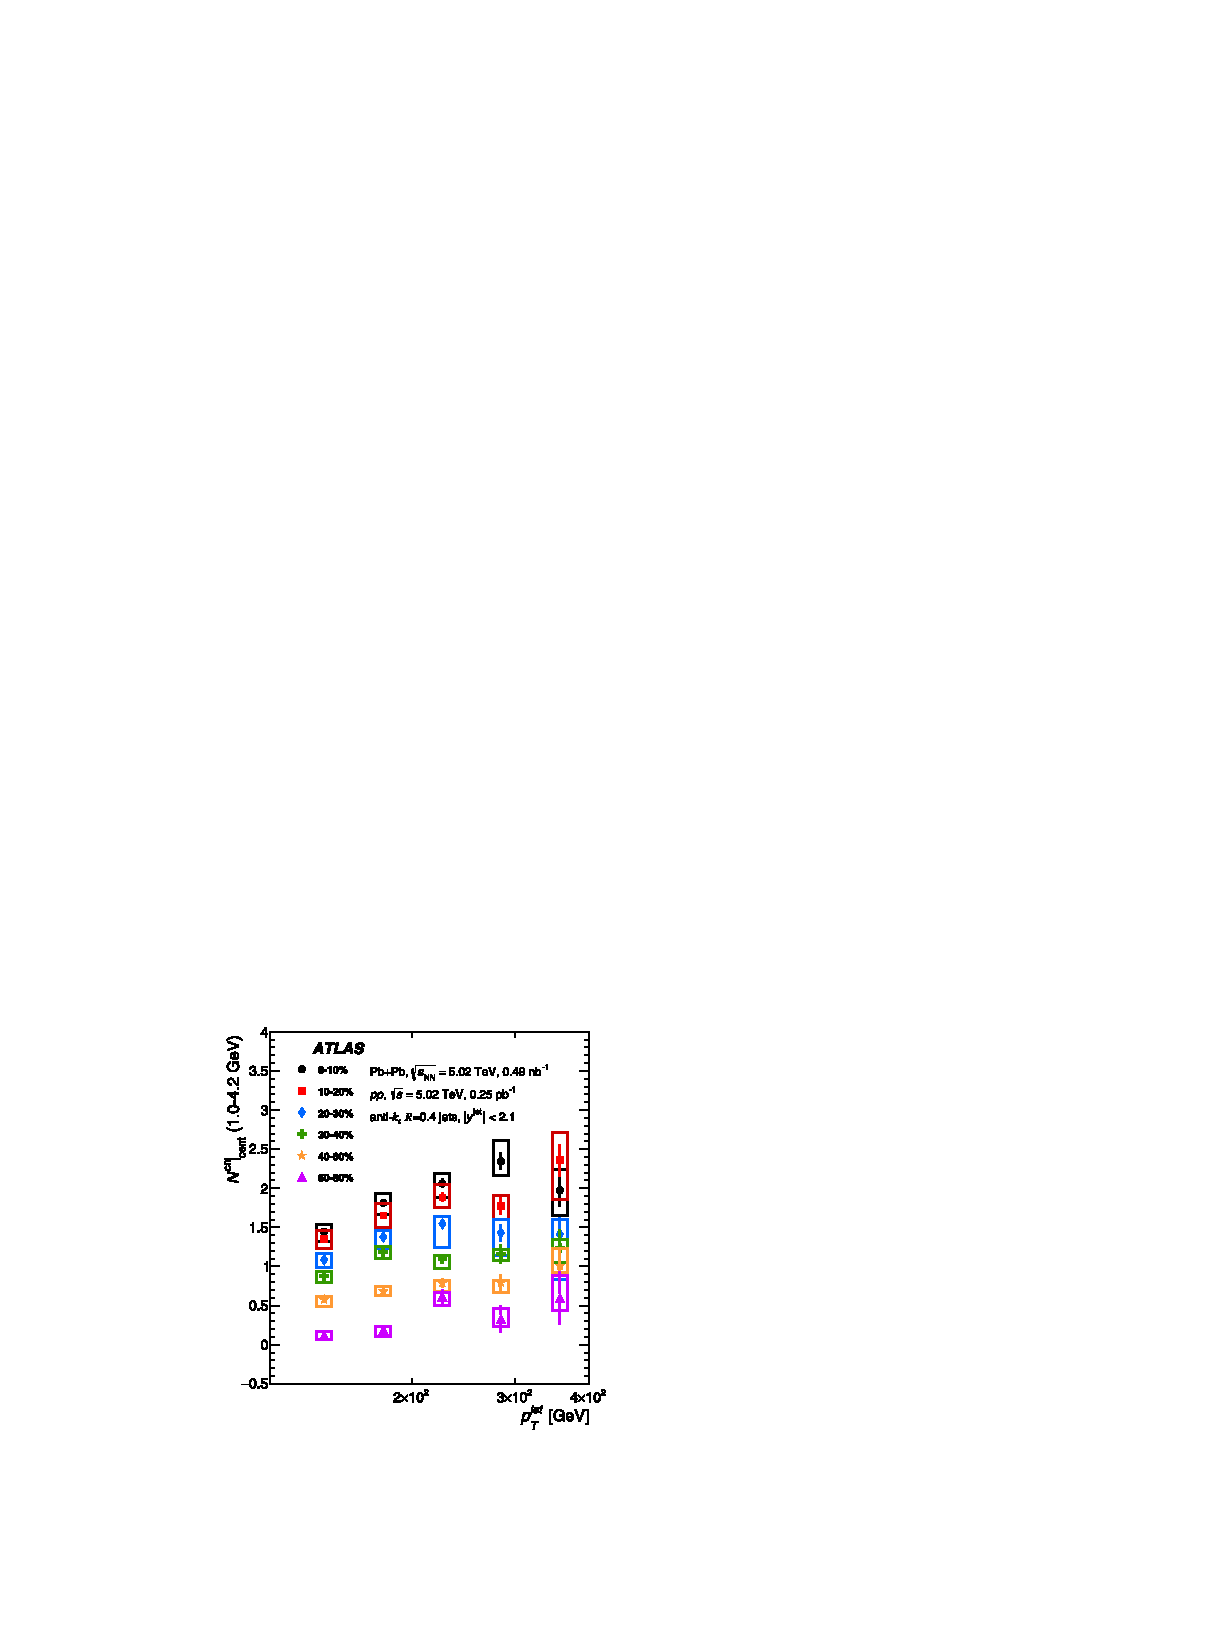
\includegraphics[width=0.35\textwidth]{figures/jetMeasurements/jetff_nch}
\caption{The number of extra particles that carry $1<\pt<4$ GeV  in \pbpb\ compared to \pp.
The different colors represent different centrality selections.
The error bars represent statistical uncertainties while the shaded boxes represent systematic uncertainties.
Figure taken from \cite{PhysRevC.98.024908}.}
\label{fig:jetff_nch}
\end{center}
\end{figure}

The modifications to the \Dz\ distributions have also been compared to a variety of models, including the Effective Quenching model \cite{Spousta:2015fca}, the Soft Collinear Effective Theory \cite{Chien:2015vja, Kang:2017frl}, and the Hybrid Model \cite{Casalderrey-Solana:2014bpa}.
These comparisons are shown in Figure~\ref{fig:jetff_rdz_theory}, and are discussed in detail in Chapter~\ref{sec:jetModels}.

\begin{figure}[htbp]
\begin{center}
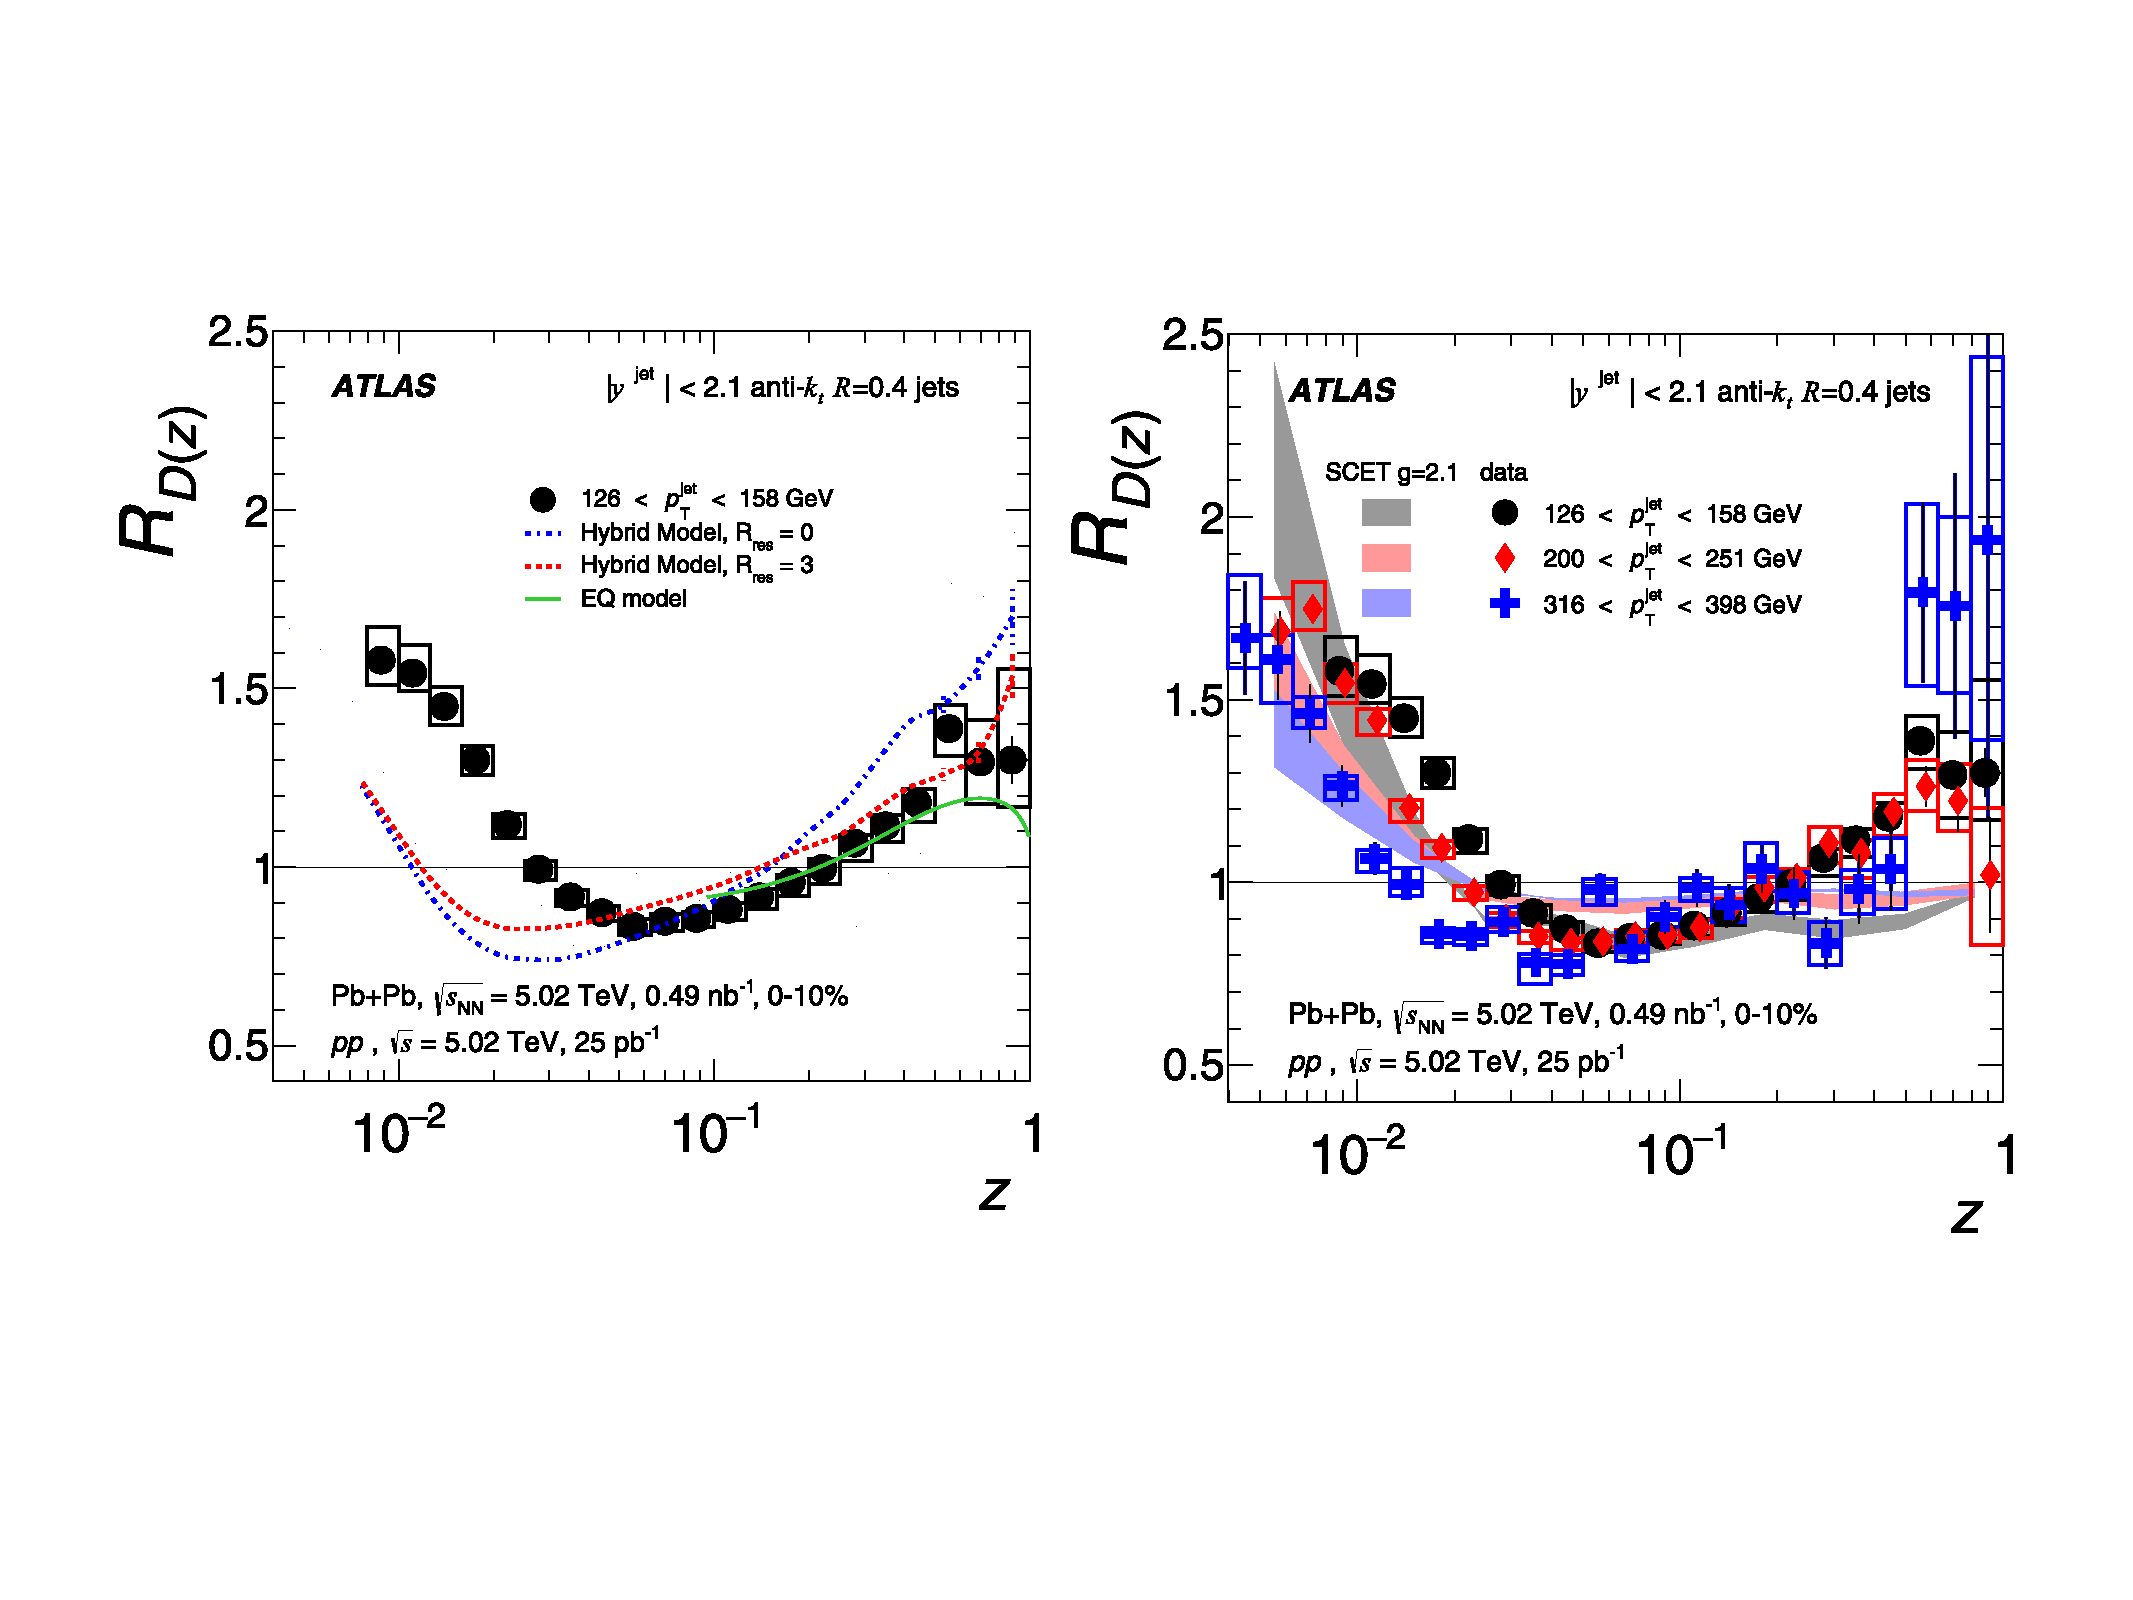
\includegraphics[width=0.75\textwidth]{figures/jetMeasurements/jetff_rdz_theory}
\caption{The \Rdz\ distributions compared to the EQ and Hybrid models (left) and SCET (right).
The error bars represent statistical uncertainties while the shaded boxes represent systematic uncertainties.
Figure taken from \cite{PhysRevC.98.024908}.}
\label{fig:jetff_rdz_theory}
\end{center}
\end{figure}





\section{Jet Profile}
\label{sec:jet_shape}
% !TEX encoding = UTF-8 Unicode
% !TEX root = thesis-ex.tex

This section will discuss the momentum profile of the jet as measured by the CMS detector for \pbpb\ collisions at $\sqrtsnn = 5.02$ TeV \cite{Sirunyan:2018jqr}.
This can be considered to be an extension to a fragmentation function measurement in that it provides information about the momentum distribution of charged particles not only within the jet boundary, but also outside.
The jet profile is defined as the distribution of particle yields in an annulus of width $\Delta r$ and is given as:

\begin{align}
%\rho(\Delta r) = \frac{1}{\sum_{\rm jets} \sum_{\rm tracks} \pTtrk} \left[ \frac{1}{\delta r} \frac{1}{\Njet} \sum\nolimits_{\rm jets}  \sum\nolimits_{{\rm tracks} \in (\Delta r_a, \Delta r_b)} \pTtrk   \right]
P(\Delta r) = \frac{1}{\delta r} \frac{1}{\Njet} \sum\nolimits_{\rm jets}  \sum\nolimits_{{\rm tracks} \in (\Delta r_a, \Delta r_b)} \pTtrk   
\end{align}
where $\Delta r_a$ and $\Delta r_b$ are the edges of the annulus at $\Delta R$, and $\delta r = \Delta r_b - \Delta r_a$.

The jet profile for \pp, \pbpb, and the modification to the jet shape variable are shown in Figure~\ref{fig:jetshape_cms}.
It can be seen from the bottom panels that there is an excess of low \pt\ particles in \pbpb\ compared to \pp\ at intermediate and large distances from the jet axis.
This enhancement is compensated by a depletion of high \pt\ particles ($\pt > 4$ GeV) at all angles.
In particular, the depletion in particle yields in 0--10\% central \pbpb\ is up to almost half the particle yields in \pp\ for $\Delta r > 0.4$.
The modifications be described in terms of jet quenching, coupled with effects from the wake the jet as it propagates through the QGP.
This wake can cause an enhancement in the low \pt\ yield of particles that is most easily seen at large angles.

\begin{figure}[htbp]
\begin{center}
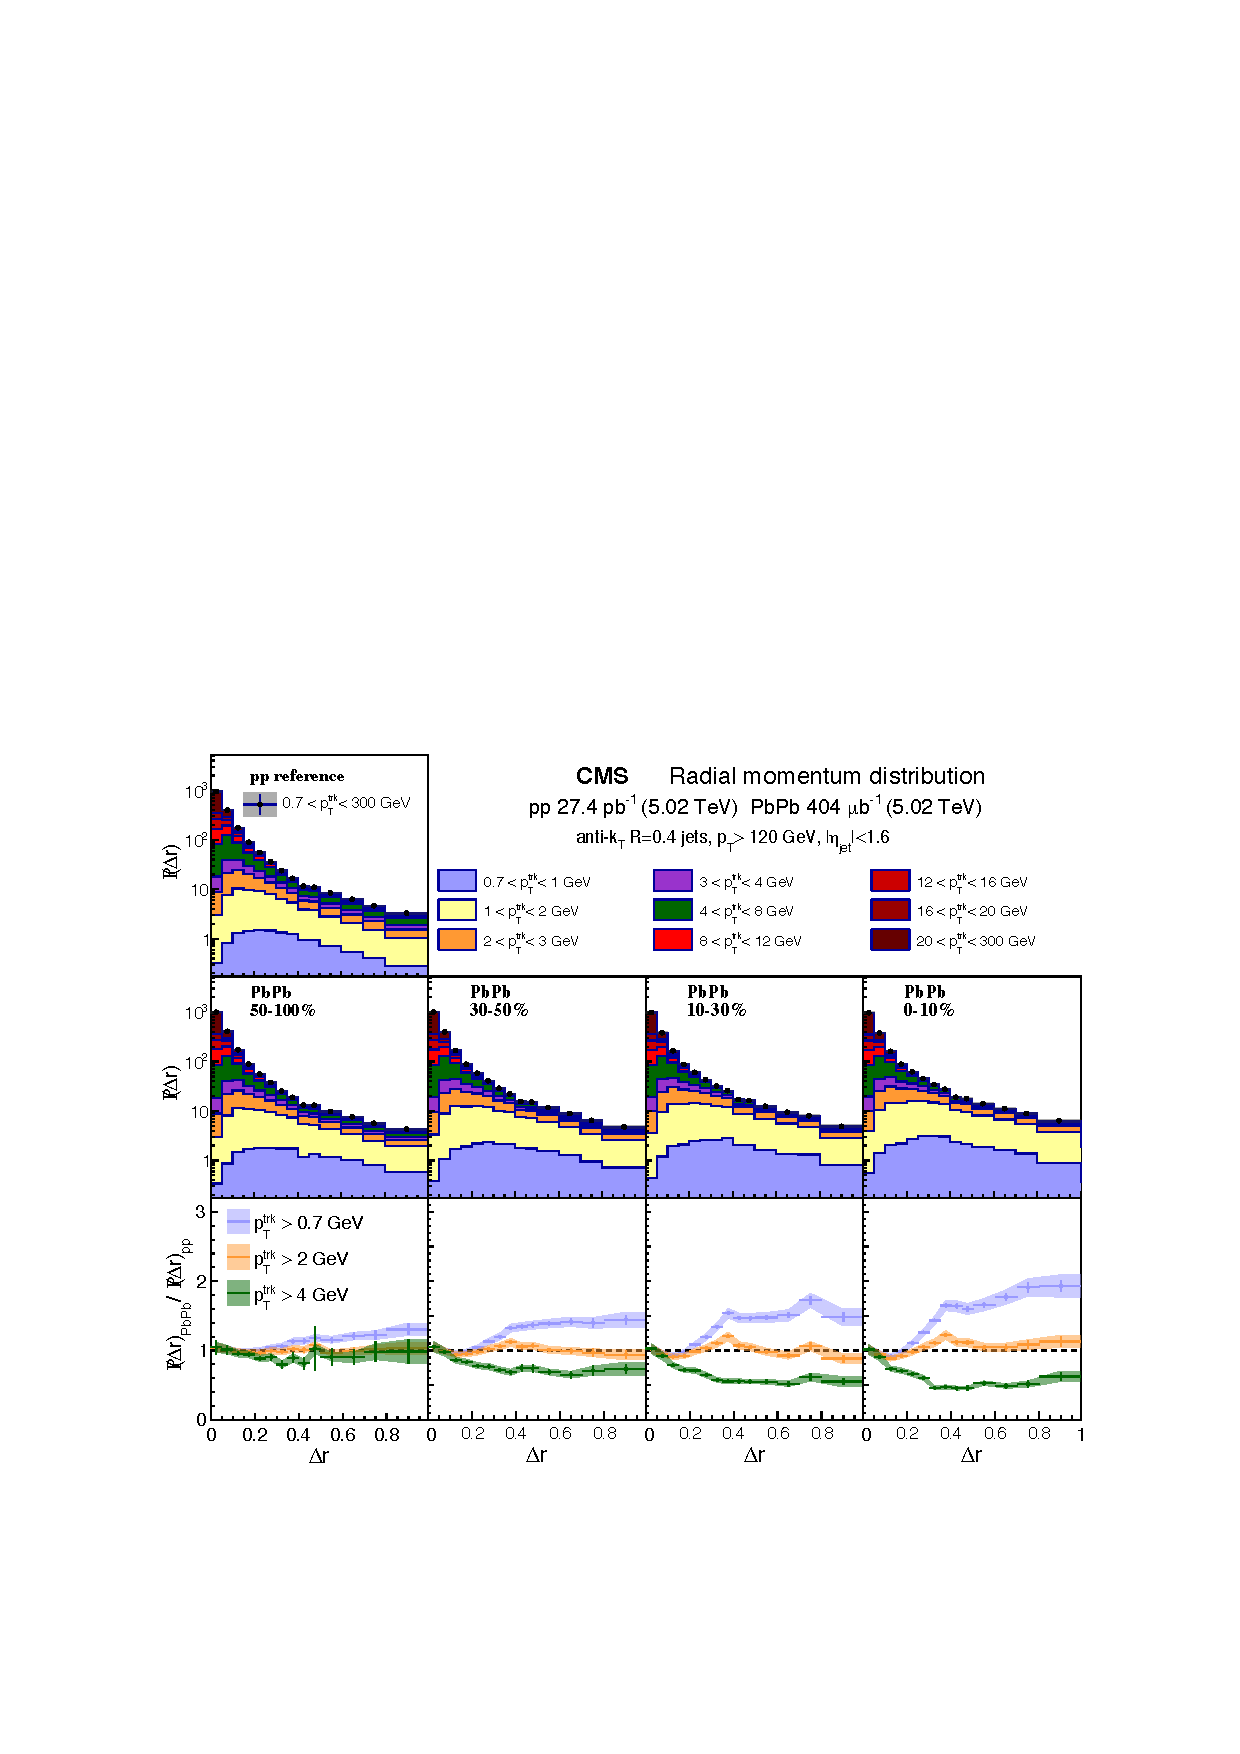
\includegraphics[width=0.75\textwidth]{figures/jetMeasurements/jetshape_cms}
\caption{The jet profile in \pp\ (top) and \pbpb\ (middle) as a function of distance from the jet axis.
The different panels in the middle give the jet shape distribution for different centrality intervals.
The modifications to the jet shape are shown at the bottom, with each panel corresponding to a different centrality.
Figure from Ref.~\cite{Sirunyan:2018jqr}.}
\label{fig:jetshape_cms}
\end{center}
\end{figure}








